\section{What we find}\label{sec:structure}

What do the groups look like on the archive, and how far do pilots depend on each other: in a pair,
in a group, between groups and from one day to the next? The groups are those
labelled by the method of the note \emph{Group flights in free flight}, with its chosen values,
$\delta=2$~min and $q=0.1$: 21.7\% of the paraglider flights and 6.9\% of the hang-glider
flights fly in a group at some point, in 17\,169 episodes (Table~\ref{gi-tab:q} of the note).
Chance is the null model of Section~\ref{gi-sec:null} of the note; bands are 5--95\% of 200 draws
of the dependency blocks, or of the dates where the captions say so. Graph terms are defined in
Appendix~\ref{app:graphs}, the two models in Appendix~\ref{app:models}. The report
\emph{Group and solo flights} (\texttt{analyses/groups/vs-solo}) compares the motion
of pilots in a group and alone; some results here refer to it. The section goes from two pilots to
the group, to what lies between groups and to the pilots across days. In short: pilots in contact
keep a shared pace and the same line, the lead passes with the thermals, the gliders around a group
add little beyond their number, and pilots come back to the same partners and clubs
(Section~\ref{sec:conclusions}).


\subsection{Two pilots}\label{sec:pilots}

Two questions about the pilots of a pair in contact. Do they keep the same pace
(Section~\ref{sec:cohesion})? And in glide, does the follower turn where the head turned or when
it turned (Section~\ref{sec:headings})?

\subsubsection{What keeps two pilots together}\label{sec:group-structure}\label{sec:cohesion}

Do two pilots in a group keep the same pace, or are they pulled back to each other? We follow the
delay $\ell^*(t)$ inside each contact (Appendix~\ref{gi-sec:lag} of the note), leaving out the instants with either
pilot in a search. Groups are the \StCohReal{} pair intervals of pilots who took off within 10~km;
chance is the \StCohChance{} contacts of the surrogate pairs, two pilots who never saw each other,
and the \StCohChanceLong{} of these that last at least $\tau^*$, selected as the groups are. Three
measures:
\begin{itemize}
  \item $D(s)=\langle(\ell(t+s)-\ell(t))^2\rangle$, the mean square change of the delay after $s$,
        fitted by an Ornstein--Uhlenbeck process, $D(s)=2\sigma^2(1-e^{-ks})+c$: $1/k$ is how long
        the delay remembers its value, $\sigma$ its spread, $2k\sigma^2$ how fast it wanders;
  \item the drift $\langle\ell(t+60~\mathrm{s})-\ell(t)\rangle/60~\mathrm{s}$ at each $\ell$, made
        symmetric since the order of a pair is arbitrary: the pull back to $\ell=0$, a spring $-k\ell$
        near 0;
  \item the distance between the two pilots at the same instant after their first contact. Two
        independent pilots separate as twice the displacement variance of one, since the drift along
        the route cancels in their difference; the surrogate pairs give this baseline on the same
        terrain.
\end{itemize}

\begin{figure}
\centering
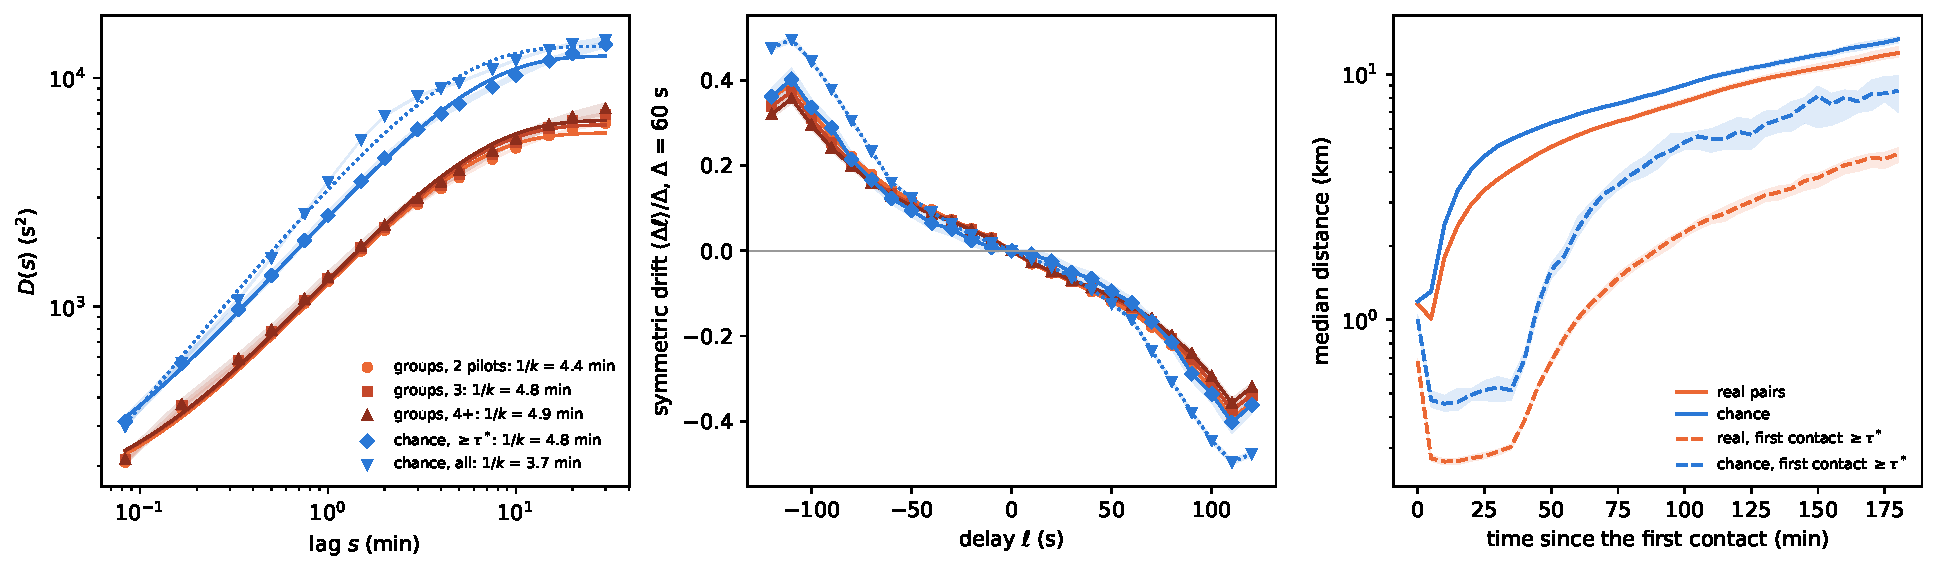
\includegraphics[width=\textwidth]{figures/structure/cohesion.pdf}
\caption{Left: $D(s)$ of groups (by size) and of chance contacts (markers), with the
Ornstein--Uhlenbeck fit (lines) and its $1/k$. Middle: symmetric drift of the delay. Right: median distance at the same
instant after the first contact, for every pair and for those whose first contact lasts at least
$\tau^*$. Bands: 5--95\% of 200 draws of the dates.}
\label{fig:cohesion}
\end{figure}

\begin{itemize}
  \item \textbf{Groups keep the same pace.} Their delay wanders at $2k\sigma^2=\StQReal$ \StQRealBand~s$^2$/s,
        against \StQChanceLong{} \StQChanceLongBand{} for chance contacts as long and \StQChance{}
        \StQChanceBand{} for all of them; its spread is $\sigma=\StSigmaReal$~s \StSigmaRealBand, against
        \StSigmaChance~s \StSigmaChanceBand. Size does not matter: $2k\sigma^2=\StQTwo$, \StQThree{} and
        \StQFour~s$^2$/s at 2, 3 and 4+ pilots.
  \item \textbf{They are not pulled back much harder.} The delay forgets itself in $1/k=\StOuReal$~min
        \StOuRealBand, against \StOuChance~min \StOuChanceBand{} by chance; the drift gives \StDriftReal~min
        \StDriftRealBand{} against \StDriftChance~min \StDriftChanceBand. Most of the pull is the
        selection: a contact that lasts keeps $|\ell|\le\delta$ by definition.
  \item \textbf{They stay together after the contact that selected them.} When the first contact lasts
        at least $\tau^*$, the two pilots are \StSepRealLongSixty~km apart 60~min later (median), against
        \StSepChanceLongSixty~km by chance; \StSepRealLongTwoHours{} against \StSepChanceLongTwoHours~km
        after 2~h. Over every first contact, \StSepRealThirty{} against \StSepChanceThirty~km after 30~min.
\end{itemize}
What holds a group together is a shared pace; a spring adds little to it. Whether the shared pace
is following or the same choices in the same air, the data cannot tell.

\subsubsection{Where and when they turn}\label{sec:headings}

Does the follower turn where the head turned, or when? In glide two pilots in contact fly along
one route, and a follower who retraces the head's track turns at the same places, a delay $\ell$
later, without seeing the head. A follower who answers the head's turns would turn within seconds
of them, whatever $\ell$. The lag of the peak of the correlation between the two headings tells the
two apart.

We take the glides of the paragraph \emph{In glide} (Section~\ref{sec:glide}), on the 5~s grid,
for the pairs of two, for every pair of members of the groups of 3 or more, and for the surrogate
pairs: \StHdGlides{} pair-glides in groups and \StHdChance{} of chance. The heading $\theta_i(t)$
of a pilot is the direction of its horizontal velocity, the displacement between the neighbouring
instants. With $\theta_{\rm route}$ the direction of the displacement of the centroid from the
start to the end of the glide and $\varphi_i$ the difference wrapped to $(-\pi,\pi]$, the pair
$(i,j)$ is oriented so that $i$ is ahead ($\ell\ge 0$, the median over the glide of $x_j-x_i$
of~\eqref{eq:passage}), and
\begin{equation}\label{eq:heading}
\varphi_i(t)=\theta_i(t)-\theta_{\rm route},\qquad
C(\tau)=\operatorname{corr}_t\big(\varphi_i(t),\,\varphi_j(t+\tau)\big),
\end{equation}
over the instants where both exist inside the glide, $\tau>0$ when $j$ follows $i$. The curves of a
class of $\ell$ are pooled over its pair-glides, as the sum of the products over the square root
of the product of the sums of squares, so a long glide weighs more. The classes are cut at
\StHdEdgeOne, \StHdEdgeTwo{} and \StHdEdgeThree~s, the quartiles of $\ell$, and $\tau$ runs to
$\pm\StHdTauMax$~s, the 95th percentile of $\ell$. We write $C(\ell)$ for the pooled $C$ read at
$\tau=\ell$ of the median $\ell$ of the class. The same is done for the horizontal speed. Chance is
the surrogate pairs, two pilots who never saw each other, in classes of $\ell$ of their own
(median delays \StHdLChanceOne, \StHdLChanceTwo, \StHdLChanceThree{} and \StHdLChanceFour~s).

\begin{figure}
\centering
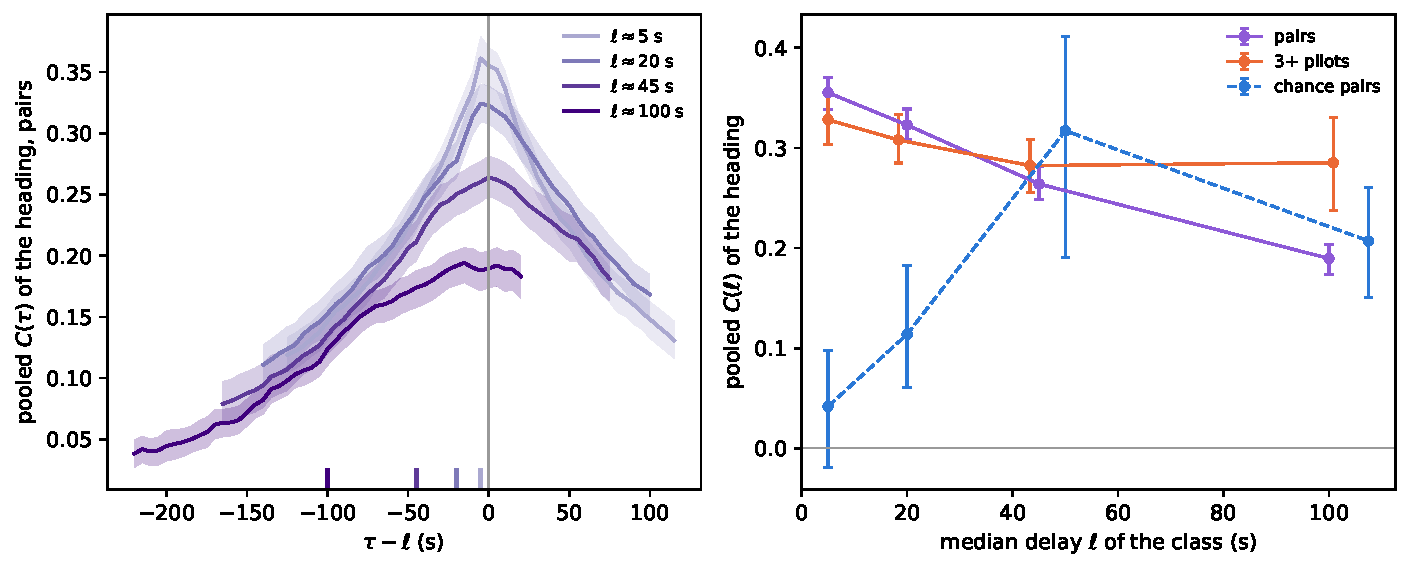
\includegraphics[width=\textwidth]{figures/structure/headings.pdf}
\caption{Headings in glide. Left: pooled $C(\tau)$~\eqref{eq:heading} of the pairs of two by class of
the median delay $\ell$, against $\tau-\ell$; a follower who retraces the head's track peaks at 0,
one who turns when the head turns at $-\ell$ (ticks). Right: pooled $C(\ell)$ against $\ell$ for
the pairs, the pairs of members of groups of 3 or more, and the surrogate pairs. Bands: 5--95\% of
200 draws of the dependency blocks (chance: of the dates).}
\label{fig:headings}
\end{figure}

\begin{itemize}
  \item \textbf{The follower turns where the head turned} (Figure~\ref{fig:headings}, left): in
        pairs the peak sits at $\tau=\StHdPeakOne$, \StHdPeakTwo, \StHdPeakThree{} and
        \StHdPeakFour~s for $\ell=\StHdLOne$, \StHdLTwo, \StHdLThree{} and \StHdLFour~s. There is no
        second peak at short $\tau$: $C(0)$ is the tail of the peak. The speed peaks at the same
        lags, within \StHdSpeedGap~s of $\ell$ in every class.
  \item \textbf{Close pilots share the line more than chance} (right): $C(\ell)$ of the pairs falls
        from \StHdCPairOne{} \StHdCPairOneBand{} at $\ell=\StHdLOne$~s to \StHdCPairFour{}
        \StHdCPairFourBand{} at \StHdLFour~s. Chance pairs give \StHdCChanceOne{}
        \StHdCChanceOneBand{} and \StHdCChanceTwo{} \StHdCChanceTwoBand{} at \StHdLChanceOne{} and
        \StHdLChanceTwo~s, but \StHdCChanceThree{} \StHdCChanceThreeBand{} and \StHdCChanceFour{}
        \StHdCChanceFourBand{} at \StHdLChanceThree{} and \StHdLChanceFour~s, as high as the pairs
        (\StHdCPairThree{} at \StHdLThree~s): far apart in time, the place alone gives the line.
  \item \textbf{In larger groups the line is kept farther} (right): between members
        \StHdLThreeFour~s apart $C(\ell)$ stays at \StHdCThreeFour{} \StHdCThreeFourBand, against
        \StHdCPairFour{} in pairs, as if each member retraced the one ahead of it.
\end{itemize}
The 5~s grid is enough to tell a delay of tens of seconds from a short one: in the classes with
$\ell$ of \StHdLTwo~s or more, a response at a short lag would be a second peak near $\tau=0$, and
there is none. Since no response appears, we do not build a directed network of who answers whom: it
would repeat the order of Section~\ref{sec:leaders}.

\paragraph{What we keep.} Pilots of a pair keep a shared pace (Section~\ref{sec:cohesion}), and in
glide they share it through the line: the follower turns at the places where the head turned, the
delay later, and shows no turn at short delays. Pairs that fly close share the line more than
chance pairs do, and at delays of \StHdLChanceThree~s and more the place alone gives as much. Retracing and
the same air give the same signal here, so the data still cannot tell following from flying in
the same air.

\subsection{The group}\label{sec:group}

How large and lasting are the groups, how are they laid out, and who leads?

\subsubsection{What the groups are}\label{sec:sizes}

How large are the groups, how long do they last, and how do they change? We count episodes and
groups (Section~\ref{gi-sec:groups} of the note) by number and by duration; an episode lasts from the start of
its first group to the end of its last, and its participants are the distinct flights it holds.

\begin{figure}
\centering
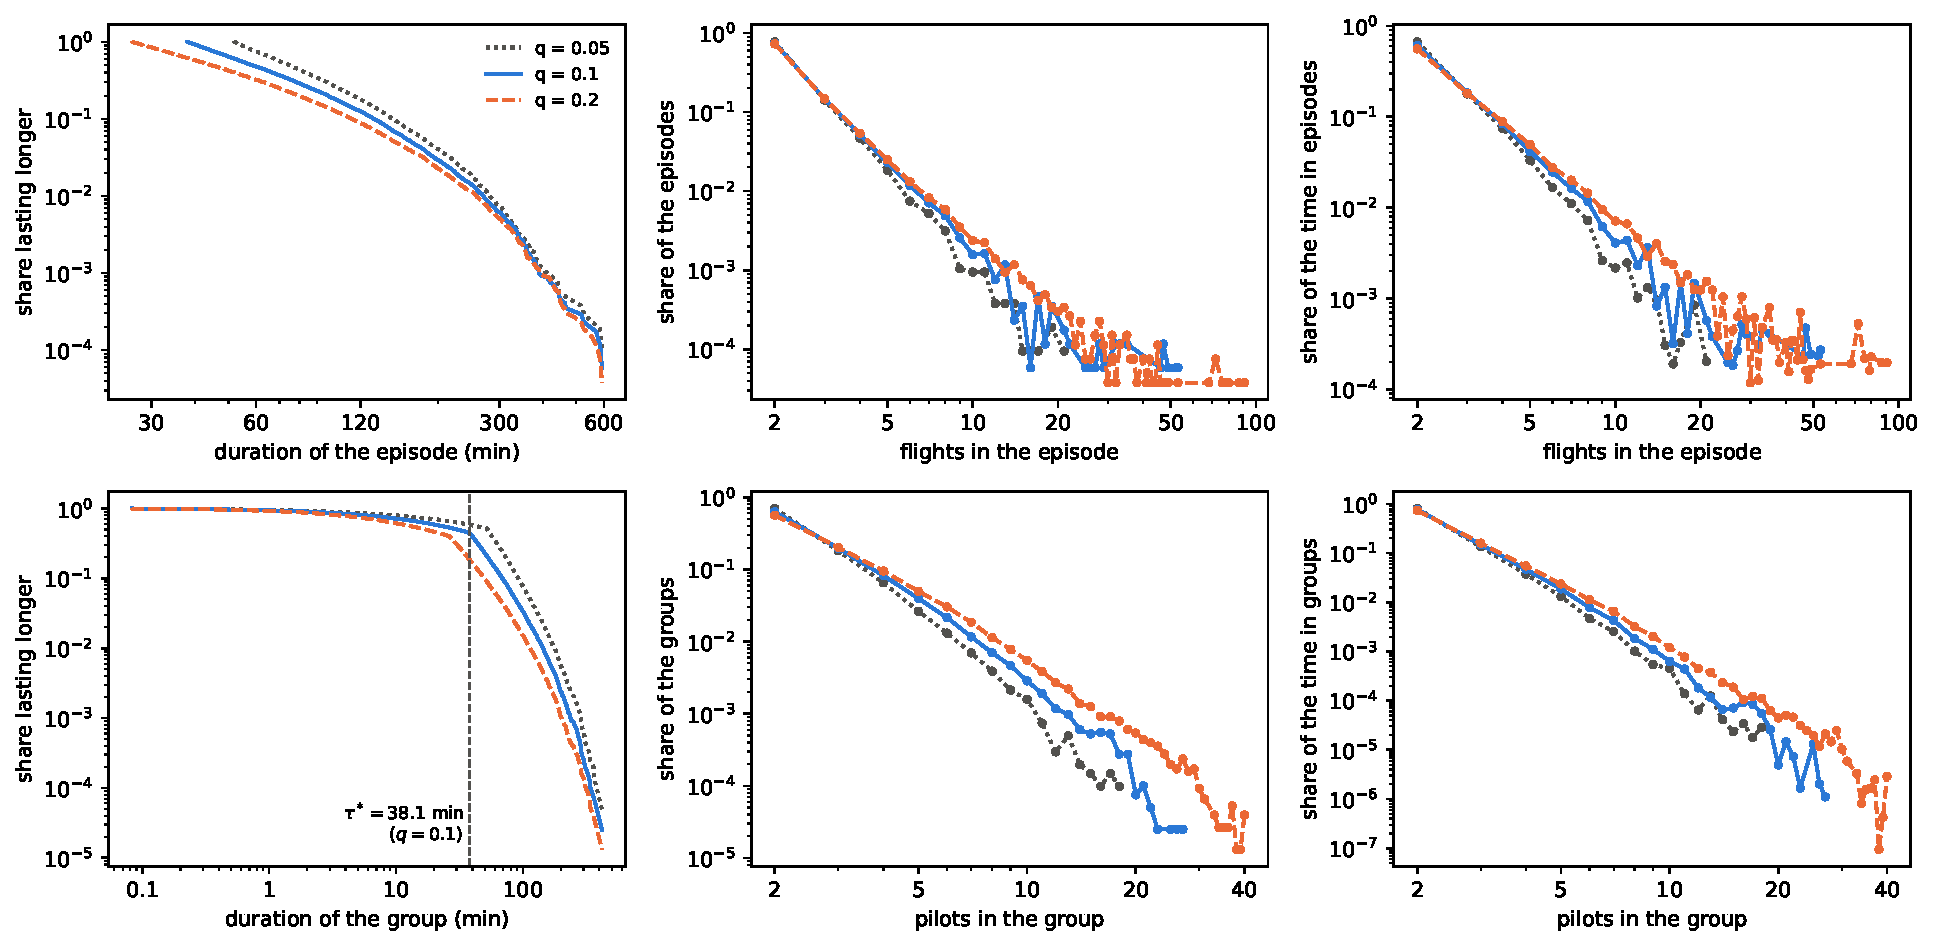
\includegraphics[width=\textwidth]{../../../methods/group-identification/figures/assessment_structure.pdf}
\caption{Episodes (top) and groups (bottom), $\delta=2$~min, whole archive, for three
values of $q$. Left: share lasting longer than a duration. Middle: share of each size. Right:
share of the total duration in each size.}
\label{fig:structure}
\end{figure}

\begin{table}
\centering
\small
\begin{tabular}{@{}l l r r c c c c r@{}}
\toprule
& $q$ & number & median & \multicolumn{2}{c}{2 participants} & \multicolumn{2}{c}{5 or more} & largest \\
& & & duration & items & time & items & time & \\
\midrule
episodes & 0.05 & 10\,553 & 74.6 min & 77\% & 67\% & 3.9\% & 8.1\% & 21 \\
 & 0.1 & 17\,169 & 58.2 min & 74\% & 61\% & 5.7\% & 12.6\% & 53 \\
 & 0.2 & 26\,504 & 44.5 min & 73\% & 56\% & 7.0\% & 17.2\% & 91 \\
\midrule
groups & 0.05 & 20\,275 & 52.7 min & 70\% & 81\% & 5.6\% & 2.3\% & 18 \\
 & 0.1 & 40\,051 & 30.4 min & 63\% & 77\% & 9.4\% & 3.5\% & 27 \\
 & 0.2 & 75\,953 & 17.1 min & 56\% & 74\% & 14.1\% & 5.0\% & 40 \\
\bottomrule
\end{tabular}
\caption{Episodes and groups for three values of $q$ ($\delta=2$~min). Items: share of the
episodes or groups of that size; time: share of their total duration.}
\label{tab:structure}
\end{table}

\paragraph{Sizes and durations.} With the chosen values the median episode lasts 58.2~min and three
in four are pairs (Table~\ref{tab:structure}). Episodes last at least $\tau^*$, since a contact
must, and larger episodes last longer, so they weigh more in time than in number. Groups have no
minimum duration: every arrival or departure of a member starts a new one, so 10\% last less
than 2.1~min, and the median is 30.4~min. Large groups change quickly, so in time the pairs weigh
more than in number. \StWithHang\% of the groups hold a hang glider. Inside a group the edges
among the members can change: the 40\,051 groups of the chosen values hold 52\,856
configurations. A larger $q$, hence a shorter $\tau^*$, gives more, shorter and larger groups:
the shares of the small sizes change little, and the tail moves.

\paragraph{How groups change.}\label{sec:describe} A group ends in one of five ways: a
\emph{join} (members added), a \emph{leave} (members removed in flight), a \emph{landing} (a
removed member lands within 5~s, the grid step), a \emph{split} or a \emph{merge}
(Appendix~\ref{app:graphs}); a group of two pilots that loses one dissolves.
Table~\ref{tab:rates} gives, by size, the groups ending per hour spent at that size.
\begin{itemize}
  \item \textbf{Most episodes never change:} \StEpisodeSingle\% of the \StEpisodes{} episodes are one
        group; \StEpisodeSplit\% hold a split, \StEpisodeMerge\% a merge.
  \item \textbf{Episodes last; groups change.} \StEpisodeTwoHours\% of the episodes last 2~h or
        more. A group lasts \StMedianGroupTwo~min with 2 pilots and \StMedianGroupMax~min with
        \StSizeMax{} or more: joins, leaves, splits and merges all grow with size, so a large group
        changes members every few minutes.
  \item \textbf{Groups break in flight:} \StEndFlight\% of the \StEnds{} groups that dissolve do
        so in flight, \StEndLanding\% at a landing; a pair ends mostly because the two separate.
        \StFormDeparture\% of the \StFormations{} groups with no predecessor form when a member
        departs: pilots who took off together.
\end{itemize}

\begin{table}
\centering
\footnotesize
\begin{tabular}{@{}r r r l l l l l@{}}
\toprule
pilots & hours & median (min) & join & leave & landing & split & merge \\
\midrule
2 & 17\,389 & 41 & 0.31\,{\tiny[0.30, 0.32]} & 0.96\,{\tiny[0.95, 0.97]} & 0.098\,{\tiny[0.094, 0.10]} & -- & 0.085\,{\tiny[0.079, 0.092]} \\
3 & 3\,349 & 20 & 0.54\,{\tiny[0.52, 0.57]} & 1.6\,{\tiny[1.6, 1.6]} & 0.050\,{\tiny[0.044, 0.056]} & -- & 0.16\,{\tiny[0.15, 0.18]} \\
4 & 1\,059 & 13 & 0.70\,{\tiny[0.66, 0.76]} & 1.6\,{\tiny[1.6, 1.7]} & 0.042\,{\tiny[0.032, 0.051]} & 0.48\,{\tiny[0.45, 0.52]} & 0.26\,{\tiny[0.22, 0.29]} \\
5 & 421 & 11 & 0.88\,{\tiny[0.80, 0.96]} & 1.7\,{\tiny[1.6, 1.8]} & 0.036\,{\tiny[0.021, 0.057]} & 0.82\,{\tiny[0.76, 0.88]} & 0.32\,{\tiny[0.26, 0.37]} \\
6 & 176 & 8 & 1.1\,{\tiny[0.93, 1.2]} & 2.1\,{\tiny[1.9, 2.3]} & 0.028\,{\tiny[0.011, 0.048]} & 1.2\,{\tiny[1.0, 1.3]} & 0.51\,{\tiny[0.40, 0.63]} \\
7 & 96 & 7 & 1.1\,{\tiny[0.91, 1.3]} & 2.0\,{\tiny[1.8, 2.2]} & 0.031\,{\tiny[0.0089, 0.074]} & 1.3\,{\tiny[1.1, 1.5]} & 0.40\,{\tiny[0.30, 0.53]} \\
8+ & 107 & 4 & 1.8\,{\tiny[1.5, 2.2]} & 2.5\,{\tiny[2.2, 2.8]} & 0.028\,{\tiny[0.0084, 0.057]} & 2.7\,{\tiny[2.4, 3.1]} & 1.0\,{\tiny[0.73, 1.2]} \\
\bottomrule
\end{tabular}

\caption{By size: hours spent, median duration of a group, and groups ending per hour by
outcome, with 5--95\% bands.}
\label{tab:rates}
\end{table}

\paragraph{Where in the flight.}\label{sec:phases} On 1~Hz flights, where the phases are labelled,
we take the phase at the instant a flight enters (\Entries{}) or leaves (\Exits{}) a group; entries
at the departure (\AtDeparture{}) and exits at the landing (\AtLanding{}) are counted apart. Both
follow the shares of the time alone in each phase (Table~\ref{tab:phases} in
Appendix~\ref{app:evidence}): there is no phase where groups preferentially form or break.
\EntriesEarly\% of the entries are within 10~min of the departure.

\paragraph{When in the day.}\label{sec:hours} Group time is concentrated around midday:
\GroupShareNoon\% of a group flight's time at \GroupShareNoonHour~h, \GroupShareMorning\% at 9~h,
\GroupShareEvening\% at 18~h (Figure~\ref{fig:hours} in Appendix~\ref{app:evidence}).

\subsubsection{Where the sizes come from}\label{sec:fission}

Why are most groups pairs, and how do a few grow large? $T(n)$ is the share of the time spent in
groups of $n$ pilots: the chance that a group seen at a random instant has $n$ pilots. If
sizes change one pilot at a time, the flux from $n$ to $n+1$ pilots balances the flux back, a
birth--death chain (Appendix~\ref{app:models}):
\begin{equation}\label{eq:chain}
  \frac{T(n+1)}{T(n)}=\frac{g(n)}{l(n+1)},
\end{equation}
with $g(n)$ the joins and $l(n)$ the leaves and landings per hour at size $n$
(Table~\ref{tab:rates}); splits and merges are left out. Per member, $g(n)=a\,n$ and
$l(n)=\mu\,n^{1-\gamma}$: every member brings in others at rate $a$ and leaves at rate
$\mu n^{-\gamma}$. We fit these to the rates, without looking at $T$. With $\gamma=0$ the chain
gives the log-series $T(n)\propto x^n/n$, $x=a/\mu$. For comparison, we fit the form of Bonabeau
et al.~\cite{bonabeau1999}, $T(n)\propto n^{-\alpha}e^{-n/n_c}$, directly to $T$.

\begin{itemize}
  \item \textbf{One pilot at a time is enough.} With the measured rates the chain gives $T(n)$ within
        4\% from 2 to 8 pilots (\StChainThreePred{} against \StChainThreeObs{} at 3 pilots, just outside
        its band), although splits and merges are \StMultiTwo\% of the changes at 2 pilots and
        \StMultiMax\% at 8+.
  \item \textbf{Members join at a constant rate and leave less often in large groups.} Each member
        brings in others at $a=\StCapitaA$ \StCapitaABand{} per hour, at every size. Each leaves at
        \StLossTwo{} per hour in a pair and \StLossMax{} at 8+: $\gamma=\StGamma$ \StGammaBand.
  \item \textbf{The heavy tail comes from staying.} With $\gamma=0$ ($x=\StX$) $T(\StNTop)$ is
        \StLogSeriesFactor{} times too small; with $\gamma=\StGamma$, \StCapitaFactor{} times. Fitted
        directly, $\alpha=\StAlpha$ and $n_c=\StNc$.
\end{itemize}

\begin{figure}
\centering
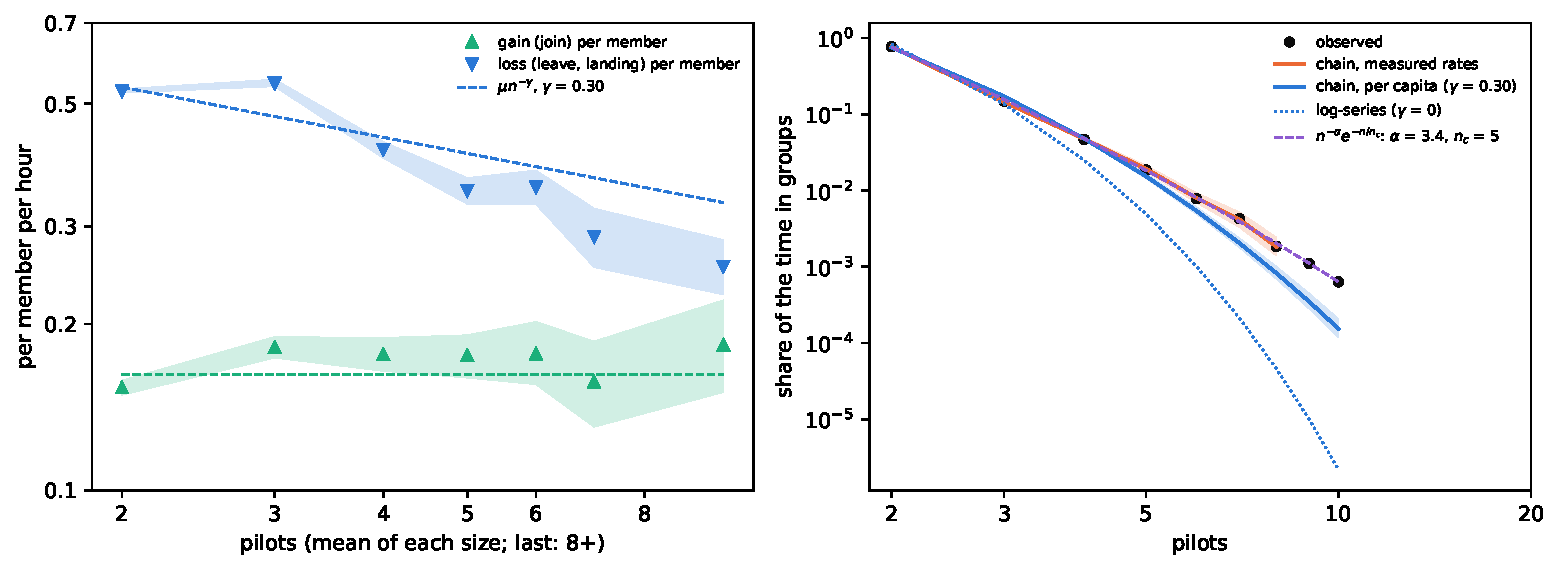
\includegraphics[width=0.9\textwidth]{figures/structure/fission.pdf}
\caption{Left: joins and losses per member per hour by size (mean size of each class; 8+ pooled),
with $a$ and $\mu n^{-\gamma}$ dashed. Right: $T(n)$ observed (sizes with at least 10~h) and from
the chain~\eqref{eq:chain} with the measured rates, with the per-capita rates and with $\gamma=0$;
dashed purple: the form of Bonabeau et al.\ fitted to $T$. Bands: 5--95\%.}
\label{fig:fission}
\end{figure}

\paragraph{The age of the episode.}\label{sec:age} The chain takes the rates as functions of the
size alone. Do they also depend on the age $a$ of the episode, the time since its start? We count
the groups of size $n$ that end with a join, a leave or a landing at age $a$, over the member-hours
spent at size $n$ and age $a$ (Figure~\ref{fig:age}). A leave, a landing or a split ends a contact,
and a contact lasts at least $\tau^*=\StTauStar$~min, so none occurs before that age: their
member-hours start there. A pilot who has just joined cannot leave for $\tau^*$ either; we keep this
time in the member-hours, which lowers the rates of young episodes, so a fall of the leaves with
age is if anything understated. Age goes with the time of day, so every rate is also taken within
three classes of local time: before 13~h, 13--15~h and after 15~h. Pairs of named paraglider pilots
are also split into those who share a contact on more than one day and the others
(Section~\ref{sec:partners}).

\begin{figure}
\centering
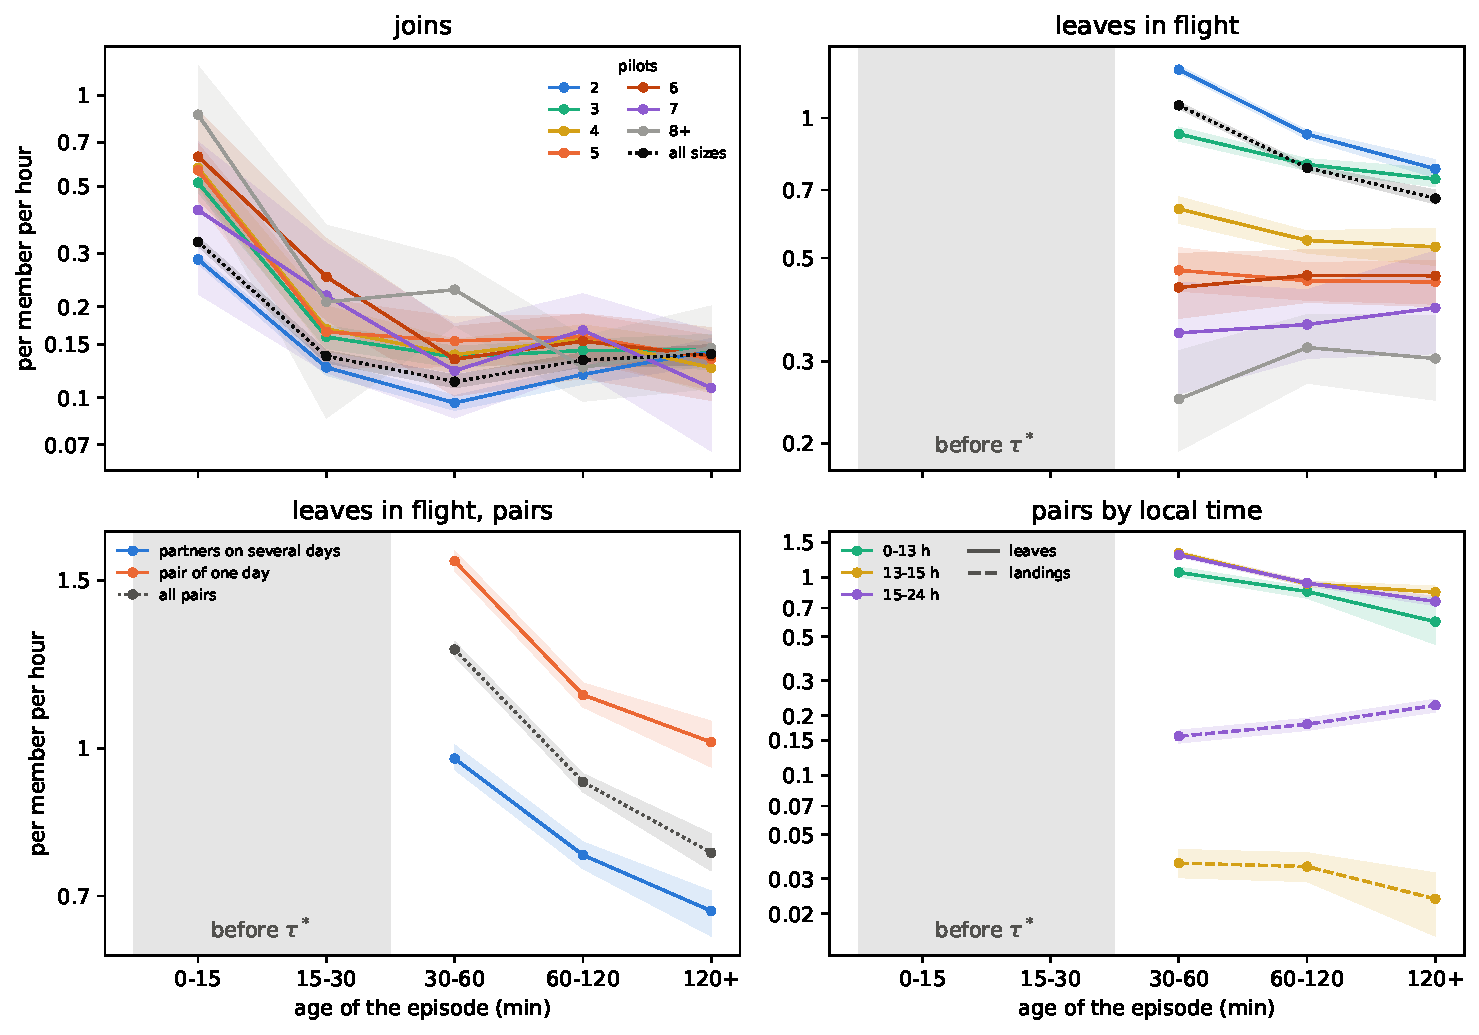
\includegraphics[width=\textwidth]{figures/structure/age.pdf}
\caption{Groups ending per member per hour against the age of the episode, with 5--95\% bands of
200 draws of the blocks. Top: joins and leaves in flight by size (dotted: all sizes), all day.
Bottom, pairs: leaves of named pilots who meet on several days and of pairs of one day; leaves
(solid) and landings (dashed) in three classes of local time. Grey: before $\tau^*$, where leaves
and landings cannot occur. Lines resting on fewer than 30 events are not drawn.}
\label{fig:age}
\end{figure}

\begin{itemize}
  \item \textbf{Joins come in the first minutes} (Figure~\ref{fig:age}, top left): in pairs
        \StAgeJoinTwoFirst{} per member per hour in the first 15~min and \StAgeJoinTwoLast{} after
        2~h, flat from 15~min on, at every size.
  \item \textbf{Pairs that have lasted separate less} (top right): from 30--60~min to 2~h and
        more their leaves fall by a factor \StAgeLeaveTwoRatio{} \StAgeLeaveTwoRatioBand; from 5
        pilots up they do not change.
  \item \textbf{Lasting partners explain a small part} (bottom left): pairs who meet on several
        days leave less, and the fall holds within each kind (factors \StAgeRepeatRatio{} and
        \StAgeOnceRatio). Other differences among pairs, such as the day or the route, may still
        select the pairs that last.
  \item \textbf{The clock moves the landings, the age the leaves} (bottom right): within each class
        of local time the leaves of pairs fall alike, while the landings rise only after 15~h.
\end{itemize}
\paragraph{What we keep.} Groups take their members in the first minutes of an episode, and
then the size moves one pilot at a time. The rates carry a memory beyond the size: a pair that has
flown together for an hour is less likely to split in the next hour than a pair that has just met,
for pilots who fly together on several days as for those who meet once. Whether flying together
binds a pair, or the pairs that last were the stable ones from the start, these data cannot tell.
The balance~\eqref{eq:chain} holds all the same, since it counts the moves between two sizes with
the rates averaged over the ages.

\subsubsection{Shape and breathing}\label{sec:shape}

How are the pilots of a group laid out, and how does the layout change along the flight?

\paragraph{Shape.}\label{sec:chains} Inside a group the members are fixed, but the pair intervals
among them start and end: each edge set is a configuration. A configuration has a density, a
diameter and a shape: complete, a tree (a chain or a star), or between (Appendix~\ref{app:graphs}).
The TA-MSD pieces of the report \emph{Group and solo flights} lie inside one group and take the
shape of its configuration at their middle.
\begin{itemize}
  \item \textbf{Large groups are strings along the route.} Three pilots form a triangle \StTriangleThree\%
        of the time and a chain \StChainThree\%. Complete graphs fall from \StCompleteFour\% of the time
        at 4 pilots to \StCompleteMax\% at 8+, the mean density from \StDensityThree{} at 3 to
        \StDensityMax{} at 8+; at 8+ the diameter is 4 or more \StDiamFourMax\% of the time: pilots
        follow each other along the route.
  \item \textbf{The shape does not change the flight.} $H_\mathrm{loc}(1000~\mathrm{s})$ is
        \StHlocTriangle{} in triangles and \StHlocChain{} in chains; \StHlocComplete{} in complete graphs
        of 4+ and \StHlocTree{} in trees. The straighter progress found in \emph{Group and solo flights}
        does not need every pilot in contact with every other.
\end{itemize}

\begin{figure}
\centering
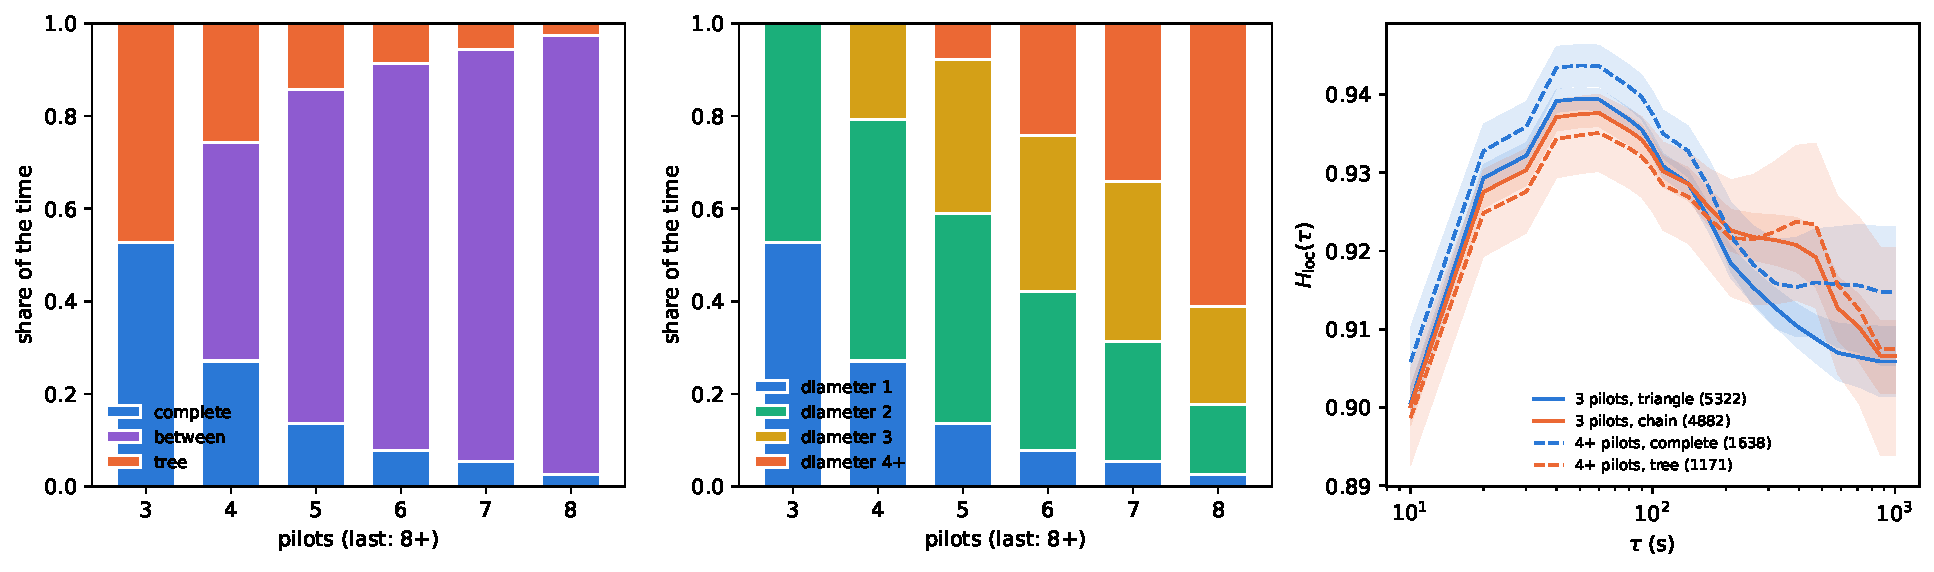
\includegraphics[width=\textwidth]{figures/structure/chains.pdf}
\caption{Left: share of the time of each shape, by size (8+ pooled). Middle: share of the time by
diameter. Right: $H_\mathrm{loc}(\tau)$ of paragliders in triangles and chains of 3 pilots, and in
complete and tree graphs of 4 or more (flights in brackets), with 5--95\% bands.}
\label{fig:chains}
\end{figure}

\paragraph{Breathing.}\label{sec:breathing} On a map a group stretches and shrinks. We follow the
groups of 2 pilots or more that last at least 30~min, all members labelled in phases
(\StBrGroups{} groups, \StBrHours~h). At each instant, with $\mathbf r_i$ the position of member
$i$, $\mathbf c$ the centroid of the members, $\hat{\mathbf u}$ the horizontal direction of the
displacement of $\mathbf c$ over 10~min (the route) and $\hat{\mathbf w}$ the horizontal direction
across it,
\begin{equation}\label{eq:lengths}
L_\parallel=\Big[\frac1n\sum_i\big((\mathbf r_i-\mathbf c)\cdot\hat{\mathbf u}\big)^2\Big]^{1/2},
\qquad
L_\perp=\Big[\frac1n\sum_i\big((\mathbf r_i-\mathbf c)\cdot\hat{\mathbf w}\big)^2\Big]^{1/2},
\end{equation}
$L_z$ is the same for the altitudes, and $f$ is the share of the members climbing. Each pilot
passes a point of the route at a time $x_i$. From the delays $\ell^*_{ij}(t)$ of the pairs in
contact, $i$ following $j$ by $\ell^*_{ij}$,
\begin{equation}\label{eq:passage}
\min_{x}\sum_{(i,j)}\big(x_i-x_j-\ell^*_{ij}(t)\big)^2,\qquad \sum_i x_i=0,
\end{equation}
over the edges of the configuration, which must connect all the members (Figure~\ref{fig:passage}). $\sigma_\ell$ is the RMS
of the $x_i$, and the head $h$ is the member of smallest $x$. If every member retraced the head's
track with its own delay, member $i$ would be where the head was a delay earlier,
\begin{equation}\label{eq:follow}
\hat{\mathbf r}_i(t)=\mathbf r_h\big(t-(x_i-x_h)\big),
\end{equation}
and $\hat L_\parallel$ follows from the $\hat{\mathbf r}_i$ as $L_\parallel$ from the $\mathbf r_i$.
At constant delays the length changes with the speed along the route alone: a head that circles in
a thermal stops on the route, and the followers close in (Figure~\ref{fig:accordion}). A group enters a thermal when $f$
reaches $1/2$ after at least 1~min at $f=0$ (Figure~\ref{fig:timeline}).

\begin{figure}
\centering
% From the delays to the passage times (left); the predicted position and the offset d (right).
\begin{tikzpicture}[x=1cm,y=1cm]
  \begin{scope}
    \draw[->, ink2] (-0.2,0) -- (4.6,0) node[right, lbl, ink] {$x$ (s)};
    \foreach \x/\n/\c in {0.6/h/blueI, 2.2/2/orangeJ, 3.8/3/aqua} {
      \draw[ink2] (\x,-0.07) -- (\x,0.07);
      \node[pt, fill=\c] (p\n) at (\x,0.95) {};
      \node[lbl, below] at (\x,-0.07) {$x_\n$};
    }
    \draw[ink2] (ph) to[bend left=45] node[above, lbl] {$\ell^*_{2h}$} (p2);
    \draw[ink2] (p2) to[bend left=45] node[above, lbl] {$\ell^*_{32}$} (p3);
    \draw[ink2, dashed] (ph) to[bend right=22] node[below, lbl] {$\ell^*_{3h}$} (p3);
    \node[note, align=center] at (2.2,-0.85) {least squares on the edges:\\ the head $h$ has the smallest $x$};
  \end{scope}
  \begin{scope}[xshift=6.6cm, scale=1.3]
    \draw[track i] (0,0.2) .. controls (1.5,0.9) and (3,0.3) .. (4.6,1.0);
    \node[pt i] at (4.6,1.0) {};
    \node[lbl, right] at (4.6,1.0) {$\mathbf r_h(t)$};
    \node[lbl, blueI, anchor=north west] at (0,0.1) {track of the head};
    \draw[->, ink2] (2.03,0.59) -- (2.93,0.62) node[right, lbl] {velocity of $h$};
    \draw[->, ink2] (2.03,0.59) -- (2.01,1.0) node[right, lbl] {$\hat{\mathbf n}$};
    \draw[orangeJ, dashed] (2.03,0.59) -- (1.93,1.95);
    \node[hollow j] at (2.03,0.59) {};
    \node[lbl, anchor=north] at (2.2,0.45) {$\hat{\mathbf r}_i=\mathbf r_h\big(t-(x_i-x_h)\big)$};
    \node[pt j] at (1.93,1.95) {};
    \node[lbl, right] at (1.98,1.95) {$\mathbf r_i(t)$};
    \node[lbl, left, orangeJ] at (1.95,1.45) {$d_i$};
  \end{scope}
\end{tikzpicture}

\caption{Left: the passage times. Each edge of the configuration carries the delay $\ell^*_{ij}$ of
a pair in contact; the $x_i$ fit them by least squares~\eqref{eq:passage}, and the head $h$ has the
smallest. Right: the predicted position~\eqref{eq:follow} of a follower, where the head was a delay
earlier, and its cross-track offset $d_i$~\eqref{eq:offset} along the unit vector $\hat{\mathbf n}$
to the left of the head's velocity there.}
\label{fig:passage}
\end{figure}

\begin{figure}
\centering
% The accordion: position along the route against time, head and follower at a constant delay.
\begin{tikzpicture}[x=1.15cm,y=0.85cm]
  \fill[blueI, opacity=0.12] (3,0) rectangle (5,5.2);
  \fill[orangeJ, opacity=0.12] (4,0) rectangle (6,5.2);
  \node[lbl, blueI] at (4,6.0) {head circles};
  \node[lbl, orangeJ] at (5,5.5) {follower circles};
  \draw[->, ink2] (0,0) -- (9,0) node[right, lbl, ink] {$t$};
  \draw[->, ink2] (0,0) -- (0,5.4) node[left, lbl, ink, align=right] {position\\along the route};
  \draw[track i] (0,0) -- (3,2.4) -- (5,2.6) -- (8,5.0);
  \draw[track j] (1,0) -- (4,2.4) -- (6,2.6) -- (8.5,4.6);
  \node[lbl, blueI, above left] at (1.9,1.5) {head};
  \node[lbl, orangeJ, below right] at (2.1,0.85) {follower};
  \draw[<->, ink] (2,1.6) -- node[above, lbl] {$\Delta$} (3,1.6);
  \draw[<->, ink] (3,2.4) -- node[below, lbl] {$\Delta$} (4,2.4);
  \draw[<->, ink] (7,3.4) -- node[right, lbl] {$v\Delta$} (7,4.2);
  \draw[ink2] (4.5,2.5) -- (4.9,3.6) node[above, note] {gap near 0};
\end{tikzpicture}

\caption{The accordion at a constant delay $\Delta$: position along the route against time. In
glide the follower is $v\Delta$ behind the head. While the head circles (blue) it stops on the
route and the follower, still gliding, closes in; while both circle the gap is near zero; it opens
again as they leave in turn. The delay $\Delta$ stays the same throughout.}
\label{fig:accordion}
\end{figure}

\begin{figure}
\centering
% A thermal of a group of three: phases of each member, the climbing share f(t), entries and exits.
\begin{tikzpicture}[x=1.2cm,y=1cm, row/.style={font=\footnotesize, anchor=east}]
  \foreach \y/\name/\climbs in {2.2/A/{2/5}, 1.5/B/{2.6/4.2,4.6/5.8}, 0.8/C/{3.1/6.2}} {
    \fill[light] (0,\y-0.15) rectangle (9,\y+0.15);
    \foreach \a/\b in \climbs {\fill[aqua] (\a,\y-0.15) rectangle (\b,\y+0.15);}
    \node[row] at (-0.1,\y) {\name};
  }
  \foreach \x/\y in {5/2.2, 5.8/1.5, 6.2/0.8} {\draw[ink, line width=0.9pt] (\x,\y-0.24) -- (\x,\y+0.24);}
  \node[lbl, above] at (2,2.35) {$t_{\rm in}$};
  \node[lbl, above] at (5,2.42) {$t_{\rm out}$};
  \begin{scope}[yshift=3.1cm]
    \draw[ink2] (0,0) -- (9,0);
    \draw[muted, dashed] (0,0.45) -- (9,0.45) node[right, lbl] {$f=1/2$};
    \draw[blueI, thick] (0,0) -| (2,0.3) -| (2.6,0.6) -| (3.1,0.9) -| (4.2,0.6) -| (4.6,0.9) -| (5,0.6)
      -| (5.8,0.3) -| (6.2,0) -- (9,0);
    \node[row] at (-0.1,0.45) {$f(t)$};
  \end{scope}
  \draw[ink, densely dotted] (2.6,0.5) -- (2.6,4.15) node[above, lbl] {entry of the group};
  \draw[decorate, decoration={brace, mirror, amplitude=4pt}, ink2] (0,0.5) -- node[below=5pt, lbl] {glide before} (1.95,0.5);
  \draw[decorate, decoration={brace, mirror, amplitude=4pt}, ink2] (2.05,0.5) -- node[below=5pt, lbl] {thermal of the group, $f>0$} (6.15,0.5);
  \draw[decorate, decoration={brace, mirror, amplitude=4pt}, ink2] (6.25,0.5) -- node[below=5pt, lbl] {glide after} (9,0.5);
  \fill[light] (9.25,2.1) rectangle (9.55,2.3); \node[lbl, right] at (9.55,2.2) {glide};
  \fill[aqua] (9.25,1.4) rectangle (9.55,1.6); \node[lbl, right] at (9.55,1.5) {climb};
\end{tikzpicture}

\caption{A thermal of a group of three pilots A, B, C. Bars: phases of each member (grey: glide,
green: climb). Top: the climbing share $f(t)$, in steps of $1/3$. The thermal of the group is the
stretch with $f>0$ between two glides of all members; the group enters it when $f$ reaches $1/2$
(dotted). Each member enters at the start of its first climb and leaves at the end of its last
(black ticks), as A at $t_{\rm in}$ and $t_{\rm out}$; B leaves once, at the end of its second
climb.}
\label{fig:timeline}
\end{figure}

\begin{figure}
\centering
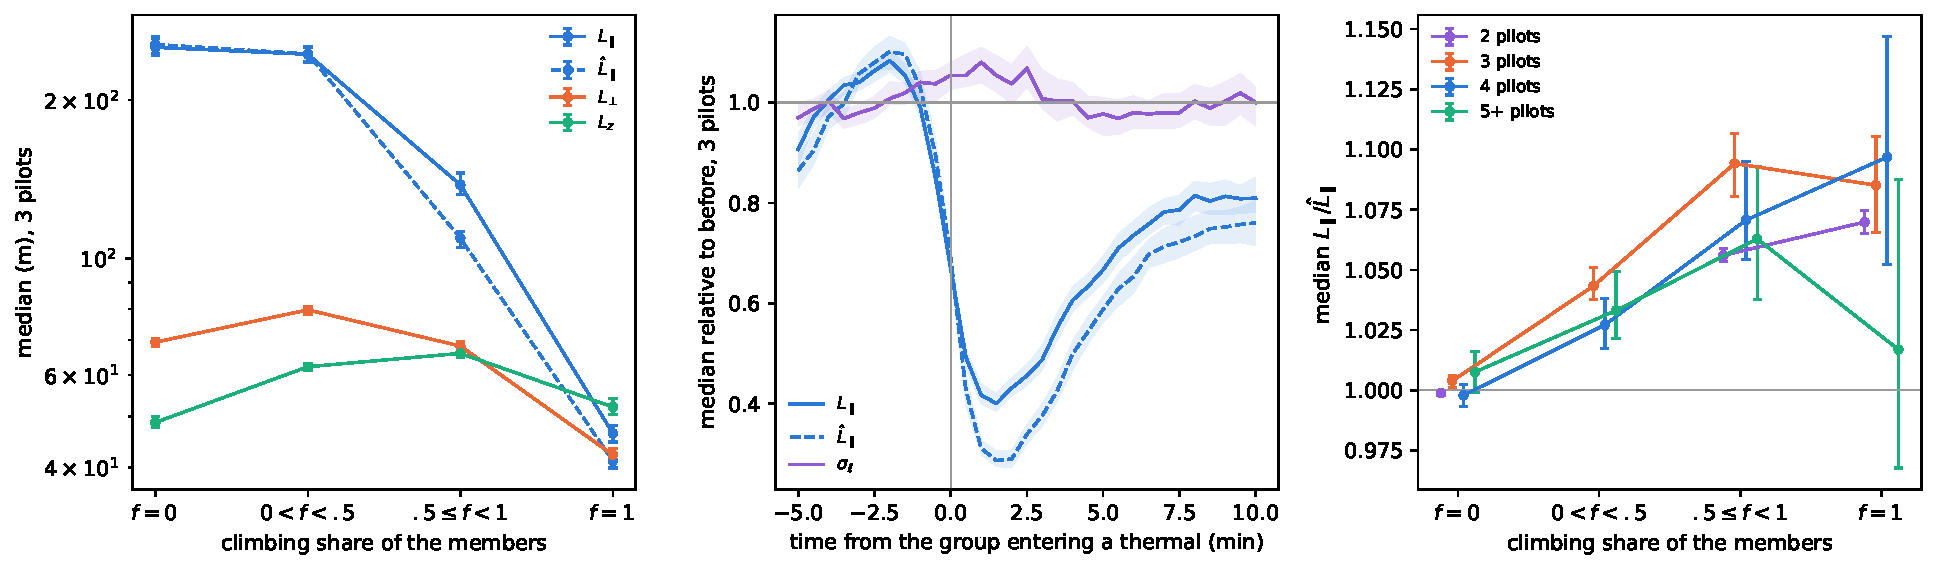
\includegraphics[width=\textwidth]{figures/structure/breathing.pdf}
\caption{Medians with 5--95\% bands of 200 draws of the blocks. Left, 3 pilots: $L_\parallel$,
$\hat L_\parallel$ (dashed), $L_\perp$ and $L_z$ in classes of the climbing share $f$. Middle, 3
pilots: $L_\parallel$, $\hat L_\parallel$ and $\sigma_\ell$ around the entry of a group in a thermal
(at 0), relative to before it. Right: $L_\parallel/\hat L_\parallel$ in classes of $f$, by size
(pairs have no $0<f<1/2$).}
\label{fig:breathing}
\end{figure}

\begin{itemize}
  \item \textbf{In a thermal the group shortens and stacks} (Figure~\ref{fig:breathing}, left): at
        3 pilots $L_\parallel$ goes from \StBrParGlide~m with all members gliding to
        \StBrParClimb~m with all climbing, while $L_z$ grows when part of the group climbs.
  \item \textbf{The delays stay} (middle): at the entry in a thermal $L_\parallel$ falls to
        \StBrEntryPar{} of its value before within 1.5~min, and $\sigma_\ell$ does not change.
  \item \textbf{Retracing the head's track explains most of it} (left and right): $\hat L_\parallel$
        follows $L_\parallel$ in every phase, with $L_\parallel/\hat L_\parallel$ at
        \StBrRatioGlide{} in glide and \StBrRatioClimb{} with all climbing at 3 pilots. The
        followers close in a little less than retracing would give, since they do not circle
        exactly where the head did. The prediction needs an order of all members,
        \StBrPredShare\% of the instants at 3 pilots.
\end{itemize}

\paragraph{In glide.}\label{sec:glide} A glide of a group is a stretch with all members gliding
($f=0$) for at least 2~min between two thermals; $s\in[0,1]$ is the time from its start over its
duration (\StGlPairs{} glides of pairs and \StGlThree{} of groups of 3 or more, median
\StGlMedian~min for pairs). Along the route, the changes of $\log L_\parallel$ over $\Delta=120$~s
split by the share of each factor $k$,
\begin{equation}\label{eq:shares}
\frac{\operatorname{Cov}(\Delta\log L_\parallel,\,\Delta\log k)}{\operatorname{Var}(\Delta\log
L_\parallel)},\qquad k=\sigma_\ell,\ v_h,
\end{equation}
with $v_h$ the speed of the head along $\hat{\mathbf u}$ over $\Delta$; at 30~s the noise of the
measurement dominates. Across the route, the offset of a follower from the head's line is
\begin{equation}\label{eq:offset}
d_i(t)=\big(\mathbf r_i(t)-\hat{\mathbf r}_i(t)\big)\cdot\hat{\mathbf n},
\end{equation}
with $\hat{\mathbf r}_i$ of~\eqref{eq:follow} and $\hat{\mathbf n}$ the horizontal unit vector to the
left of the head's velocity at that point. Chance is the same offset for the surrogate pairs whose
contact lasts at least $\tau^*$, on the glides they share, the pilot ahead taken as head
(\StGlChance{} glides; bands over the dates).

\begin{figure}
\centering
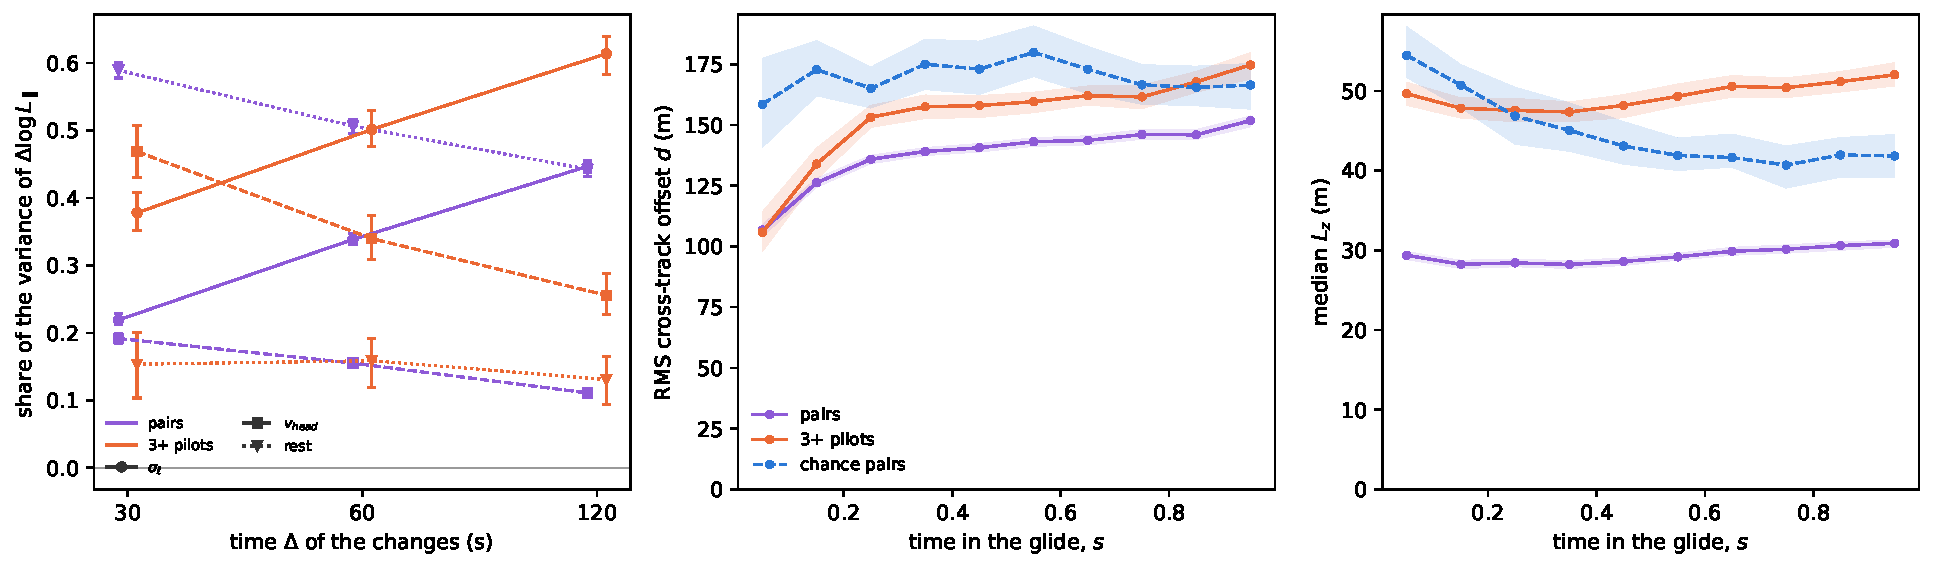
\includegraphics[width=\textwidth]{figures/structure/glide.pdf}
\caption{Glides of groups. Left: share~\eqref{eq:shares} of the variance of the changes of
$\log L_\parallel$ over $\Delta$ carried by $\sigma_\ell$, by $v_h$ and by neither, against
$\Delta$. Middle: RMS of the cross-track offset $d$ against the time $s$ in the glide, groups and
chance pairs. Right: median $L_z$ against $s$. Bands: 5--95\% of 200 draws of the blocks (chance:
of the dates).}
\label{fig:glide}
\end{figure}

\begin{itemize}
  \item \textbf{Along the route the delays move} (Figure~\ref{fig:glide}, left): $\sigma_\ell$
        carries \StGlSigmaPairs{} of the variance in pairs and the head's speed \StGlVPairs: a group
        stretches in glide mostly because a pilot gains or loses time on the others.
  \item \textbf{Across the route the group opens and stays open} (middle): the RMS of $d$ in pairs
        grows from \StGlDPairsStart~m at the start of the glide to \StGlDPairsMid~m at mid-glide and
        does not close before the next thermal. Near $s=0$ the offset needs the head's passage
        inside the glide, which favours the followers close behind.
  \item \textbf{Groups hold closer lines than chance pairs} (middle): pairs over chance is
        \StGlRatioStart{} \StGlRatioStartBand{} at the start and \StGlRatioEnd{}
        \StGlRatioEndBand{} at the end of the glide.
  \item \textbf{Height holds} (right): in glide $L_z$ stays between \StGlZPairsLow{} and
        \StGlZPairsHigh~m in pairs.
\end{itemize}
\paragraph{What we keep.} A group keeps its spacing in time, and its spacing in space follows.
In a thermal the head stops to circle and the others reach it, so the group shrinks to a few tens
of metres along the route and stacks in height; in glide it stretches again to the length its
delays give at glide speed. On a map the group breathes with the thermals, while its delays, the
quantity that holds two pilots together (Section~\ref{sec:cohesion}), barely move: the breathing is
the kinematics of a shared pace. What changes in glide is the line. After a thermal the followers
drift off the head's line and stay off it, closer to it than two pilots who never met, and the
length changes because a pilot gains or loses time on the others. We find no fan that opens across
the route to search and closes before the next thermal.

\subsubsection{Who leads}\label{sec:leaders}

Who is ahead in a group, how often does that change, and who is it?

\paragraph{Order.} The signed median delay $\ell_{\rm med}$ of a pair interval
(Appendix~\ref{gi-sec:lag} of the note) says who passes first: the pilot ahead, when the other passes at least
15~s later; otherwise the two fly abreast (\Abreast\% of the pairs of two; median delay
\DelayMedian~s). How leading changes the flight is in \emph{Group and solo flights}; here we ask
who leads (Figure~\ref{fig:hierarchy}; Figure~\ref{fig:habitual} in Appendix~\ref{app:evidence}).
\begin{itemize}
  \item \textbf{Pilots are in a line.} In groups of 3 pilots or more, each edge points from
        the pilot ahead to the one behind; we compare with the same graphs with each direction drawn
        at random (50 draws). Directed triangles are cyclic \StCyclic\% \StCyclicBand{} of the time,
        against \StCyclicNull\% at random; graphs with every edge directed (\StFullShare\% of the time)
        are acyclic \StAcyclic\%, against \StAcyclicNull\%. Positions along one route cannot form
        cycles, so the order is geometry and says nothing about rank.
  \item \textbf{One leader, in small groups:} \StOneLeader\% \StOneLeaderBand{} of the acyclic time,
        against \StOneLeaderNull\% \StOneLeaderNullBand{} at random; \StOneLeaderThree\% at 3 pilots,
        \StOneLeaderFour\% at 4, \StOneLeaderFive\% at 5 or more. A single file (depth $n-1$):
        \StLineThree, \StLineFour{} and \StLineFive\%.
  \item \textbf{The lead changes often.} Along $\ell^*(t)$, with stretches shorter than 60~s dropped,
        the pilot ahead changes \StSwitches{} times per hour of contact \StSwitchesBand{}, against
        \StSwitchesChance{} \StSwitchesChanceBand{} in chance contacts lasting at least $\tau^*$; the
        pilot most often ahead holds \StDominant\% of the directed time (median), against
        \StDominantChance\%.
  \item \textbf{The experienced pilot on the faster wing leads.} In groups of two named
        pilots, the leader has more earlier flights in the catalog in \StExp\% \StExpBand{} of
        \StExpPairs{} pairs (\StExpRatio{} times as many, median), and the higher wing class (A~=~1 to
        competition~=~5) in \StWing\% \StWingBand{} of \StWingPairs.
  \item \textbf{Some pilots lead or follow persistently.} For the \HabitualPilots{} pilots with at
        least 10 roles in pairs, the dispersion of their lead fractions is \HabitualDispersion{}
        against \HabitualNull{} with roles swapped at random (95\% below \HabitualNullHigh);
        \HabitualExtreme\% lead in at most 20\% or at least 80\% of their roles, against
        \HabitualExtremeNull\% expected.
\end{itemize}

\begin{figure}
\centering
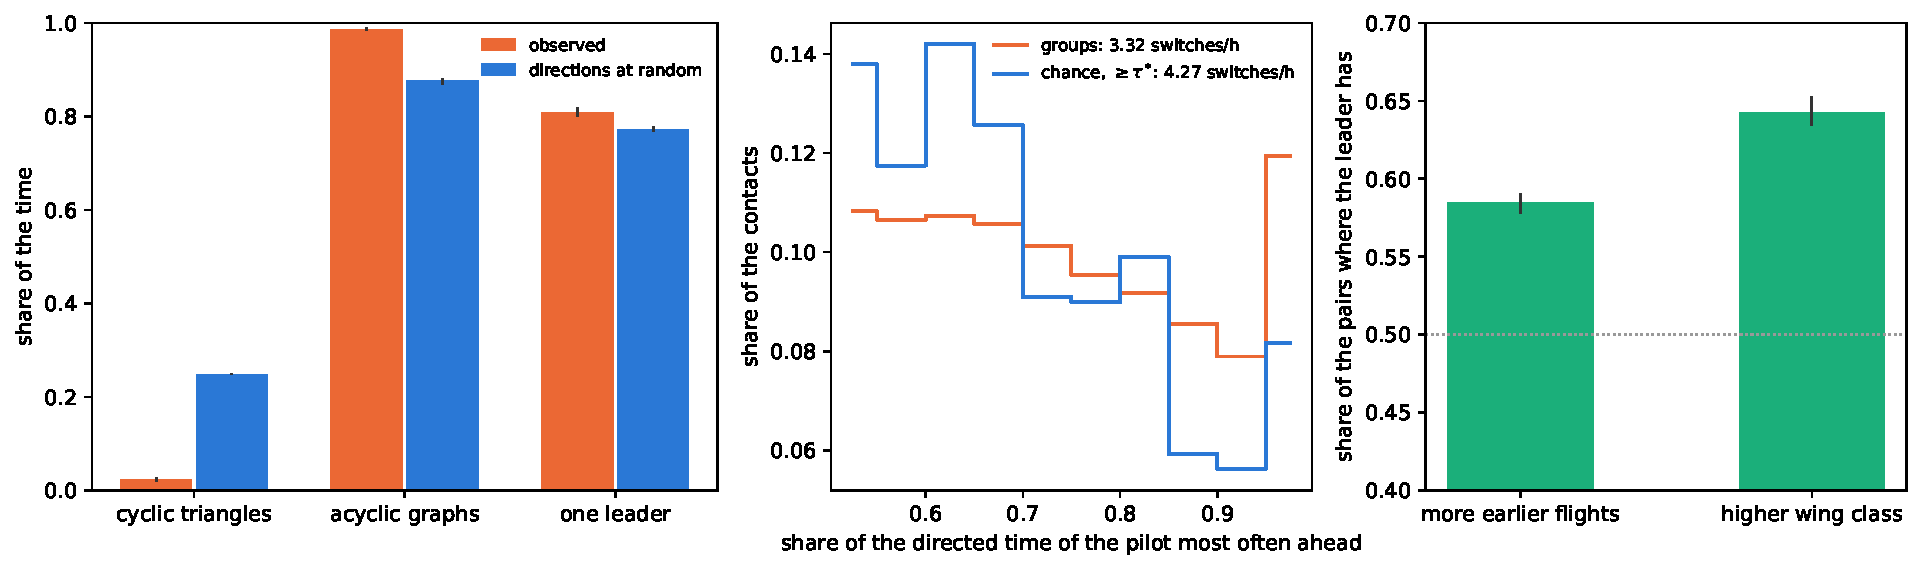
\includegraphics[width=\textwidth]{figures/structure/hierarchy.pdf}
\caption{Left: in groups of 3 or more, share of the time with cyclic directed triangles, acyclic
graphs (every edge directed) and one leader (acyclic graphs), observed and with directions at
random. Middle: share of the directed time of the pilot most often ahead in each contact, with the
switches per hour. Right: share of the pairs of two in which the leader has more earlier flights,
or the higher wing class. Bars: 5--95\% (blocks).}
\label{fig:hierarchy}
\end{figure}

\paragraph{Rotation.}\label{sec:rotation} Does the pilot ahead stay ahead? We follow the groups of
3 pilots or more that last at least 30~min, all members labelled in phases (\StRotGroups{} groups,
\StRotHours~h, with an order \StRotOrdered\% of the time). The order at $t$ ranks the passage
times $x_i$ of~\eqref{eq:passage}, head first. Its memory is the Kendall $\tau$ of the orders at
$t$ and $t+s$,
\begin{equation}\label{eq:kendall}
\tau(s)=\Big\langle\frac{2}{n(n-1)}\sum_{i<j}\operatorname{sgn}\big(x_i(t)-x_j(t)\big)\,
\operatorname{sgn}\big(x_i(t+s)-x_j(t+s)\big)\Big\rangle_t,
\end{equation}
1 for the same order and 0 for independent orders. A head spell is a run of one head, with runs
shorter than 60~s dropped as for the switches above; chance keeps the spells and draws each new
head among the other members.

\begin{figure}
\centering
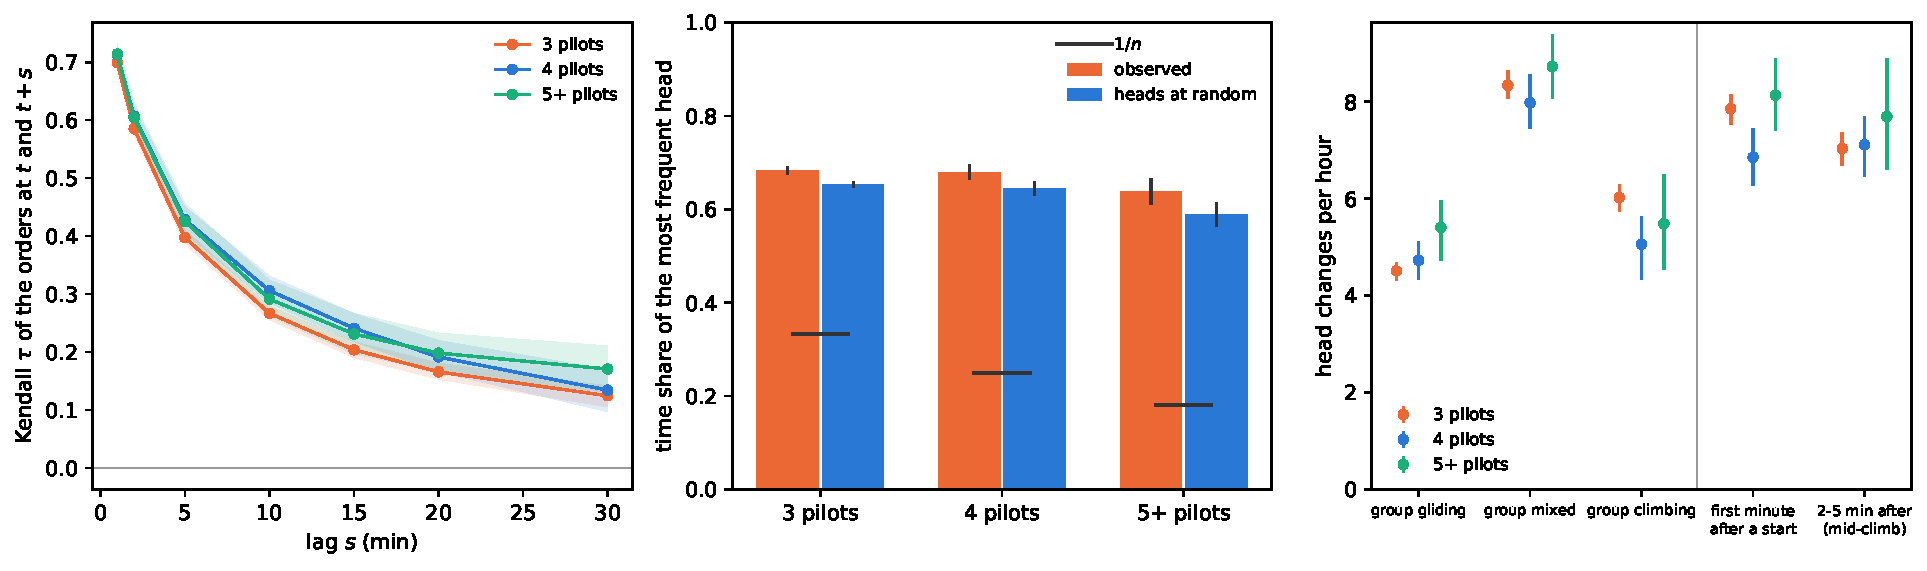
\includegraphics[width=\textwidth]{figures/structure/rotation.pdf}
\caption{Groups of 3 pilots or more lasting at least 30~min. Left: Kendall
$\tau$~\eqref{eq:kendall} of the orders at $t$ and $t+s$ against $s$, by size. Middle: time share
of the most frequent head, observed and with heads at random, with $1/n$. Right: head changes per
hour by phase of the group (all gliding, some climbing, all climbing) and, at the starts of
climbs, in the first minute against mid-climb. Bands and bars: 5--95\% of 200 draws of the
blocks.}
\label{fig:rotation}
\end{figure}

\begin{itemize}
  \item \textbf{The order renews in minutes} (Figure~\ref{fig:rotation}, left): $\tau$ falls from
        \StRotTauOne{} at 1~min to \StRotTauFifteen{} at 15~min, alike at every size, and keeps a
        weak lasting part (\StRotTauThirty{} at 30~min).
  \item \textbf{No lasting head} (middle): in groups of 3 the pilot most often ahead holds
        \StRotDominant\% of the time, against \StRotDominantNull\% with random hand-overs; the
        head changes \StRotChanges{} times per hour.
  \item \textbf{The head changes while the group straddles a thermal} (right): \StRotMixed{}
        changes per hour with some members climbing, against \StRotGliding{} with all gliding and
        \StRotClimbing{} with all climbing. The noise of $\ell^*$ is largest with all members
        circling (end of the section), so the excess is not that noise alone. The start of a climb
        adds little (\StRotFirstOverMid{} times the changes of mid-climb), and the new head is the
        first to climb in \StRotFirst\% of the changes, against \StRotFirstExp\% at random.
\end{itemize}

\paragraph{Leaving a thermal.}\label{sec:exits} Do the followers leave a thermal at the height of
the leader, below it or above it? A thermal of a group is the stretch between two glides of the
whole group, all members gliding for at least 1~min. Each member that climbs there enters at the
start of its first climb and leaves at the end of its last, at the heights $z_{\rm in}$ and
$z_{\rm out}$ and the times $t_{\rm in}$ and $t_{\rm out}$. The leader $l$ is the pilot most often
ahead (smallest $x$) in the glide before the thermal; for each follower $i$,
\begin{equation}\label{eq:exit}
\Delta z=z_{{\rm out},i}-z_{{\rm out},l},\qquad
\Delta t=t_{{\rm out},i}-t_{{\rm out},l},\qquad
\Delta g=(z_{\rm out}-z_{\rm in})_i-(z_{\rm out}-z_{\rm in})_l .
\end{equation}
The same height means $|\Delta z|\le 20$~m, about ten times the altitude noise of a fix. An offset
between two loggers enters $\Delta z$ and cancels in $\Delta g$. Chance draws the leader among the
pilots who climb there. There are \StExThermals{} thermals with two pilots climbing or more and
\StExRows{} followers; the leader of the glide after the thermal gives the same picture
(Figure~\ref{fig:exits}).

\begin{figure}
\centering
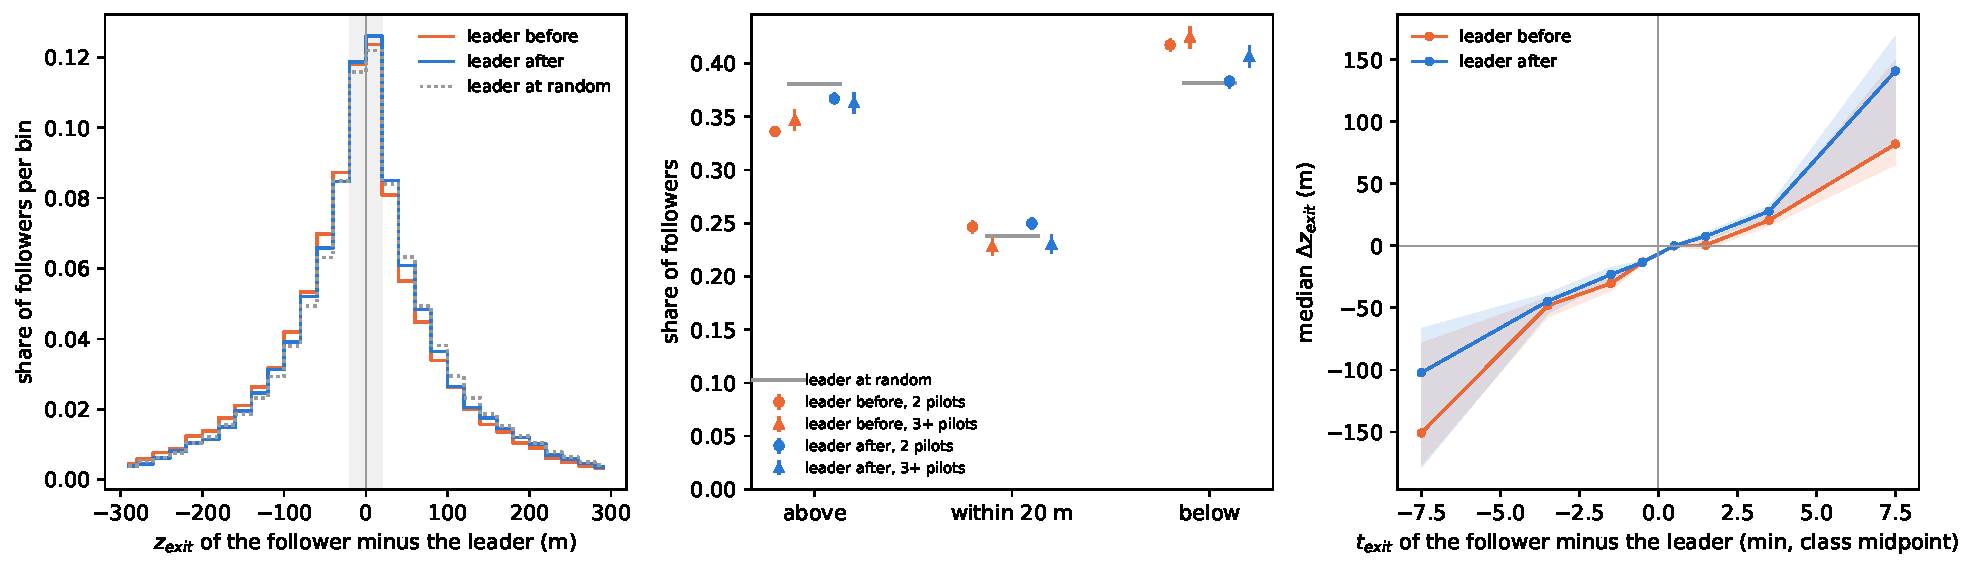
\includegraphics[width=\textwidth]{figures/structure/exits.pdf}
\caption{Followers against the leader of the glide before the thermal (orange) and of the glide
after it (blue). Left: distribution of $\Delta z$~\eqref{eq:exit} (grey: within 20~m), and with the
leader drawn at random (dotted). Middle: share of the followers leaving above the leader, within
20~m and below, by size, and with a leader at random (grey). Right: median $\Delta z$ in classes
of $\Delta t$. Bands and bars: 5--95\% of 200 draws of the blocks.}
\label{fig:exits}
\end{figure}

\begin{itemize}
  \item \textbf{Followers leave at the leader's height} (left): the median $\Delta z$ is \StExDz~m
        \StExDzBand, and the follower gains \StExDgain~m \StExDgainBand{} less than the leader,
        so the few metres are not an offset of the loggers. The spread is as wide as with a leader
        at random.
  \item \textbf{Slightly more often below} (middle): \StExBelow\% leave more than 20~m below the
        leader and \StExAbove\% above, against \StExRandomSide\% each with a leader at random.
  \item \textbf{Who stays longer leaves higher} (right): $\Delta z$ grows with $\Delta t$ on both
        sides; the follower leaves later than the leader in \StExLater\% of the cases.
  \item \textbf{Leaving first leads the next glide, leaving highest does not.} The first to leave
        is the head of the next glide in \StExFirstHead\% of the thermals, the highest in
        \StExHighHead\%, against \StExHeadExp\% at random. The first result is close to the
        definition of the head, the first to pass; the second says that height bought in the
        thermal does not buy the lead.
\end{itemize}

\paragraph{Turning in the thermal.}\label{sec:turning} Does the leader explore the thermal while
the followers settle into a steady circle? In white storks the birds that lead keep adjusting their
circle, with a larger rate of change of the curvature of the horizontal path, and the followers
circle more regularly~\cite{flack2018}. On the native 1~Hz fixes of each pilot, inside its climb in
a group thermal, the positions $(x,y)$ smoothed by a Savitzky--Golay filter over \StCuSG~s give the
signed curvature, and its rate of change $\dot\kappa$ compares a follower $i$ with the leader $l$ of
the glide before the thermal:
\begin{equation}\label{eq:curvature}
\kappa=\frac{\dot x\ddot y-\dot y\ddot x}{(\dot x^2+\dot y^2)^{3/2}},\qquad
r=\log_{10}\frac{\operatorname{med}|\dot\kappa_i|}{\operatorname{med}|\dot\kappa_l|},
\end{equation}
the medians over at least \StCuMinSec~s of climb, without the instants slower than
\StCuVmin~m/s. Two windows: each pilot's whole climb in the thermal, and the seconds where both
climb, which leave out the time one of the two spends alone centring the thermal. The circles have
a median radius of \StCuRadius~m and a turn lasts \StCuPeriod~s; there are \StCuRows{} followers in
\StCuThermals{} thermals.

\begin{figure}
\centering
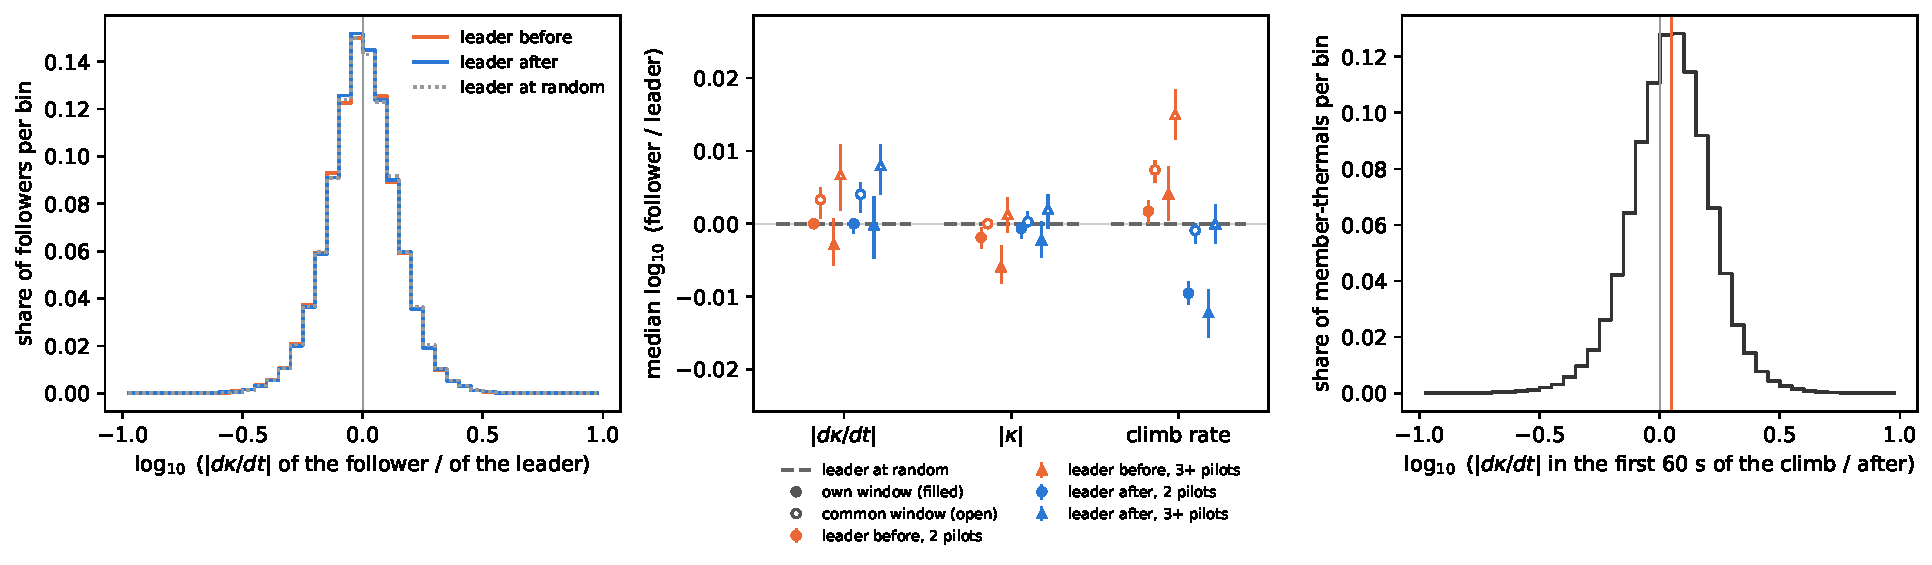
\includegraphics[width=\textwidth]{figures/structure/curvature.pdf}
\caption{Rate of change of the curvature of followers and leaders in group thermals. Left:
distribution of $r$~\eqref{eq:curvature} over each pilot's whole climb, with the leader of the
glide before (orange), after (blue) and at random (dotted). Middle: median $r$ of $|\dot\kappa|$, of
$|\kappa|$ and of the climb rate, over each pilot's whole climb (filled) and over the seconds where
both climb (open), by size. Right: $\log_{10}$ of $|\dot\kappa|$ in the first 60~s of a climb over
the rest, every climber. Bars: 5--95\% of 200 draws of the blocks.}
\label{fig:curvature}
\end{figure}

\begin{itemize}
  \item \textbf{Leaders and followers turn alike} (left): the median $r$ is \StCuR{} \StCuRBand{}
        (\StCuAfterR{} \StCuAfterRBand{} with the leader after), and the leader has the larger
        $|\dot\kappa|$ in \StCuShare\% \StCuShareBand{} of the pairs, against \StCuShareRandom\%
        with a leader at random. A filter of 5 to 11~s and a speed threshold of 2 to 5~m/s move the
        median $r$ by \StCuSensMax{} at most. We do not observe what Flack et
        al.~\cite{flack2018} observe in storks.
  \item \textbf{While both climb, the follower turns slightly more} (middle): its $|\dot\kappa|$ is
        \StCuCommon\% \StCuCommonBand{} higher, and the leader's is the larger in
        \StCuCommonShare\% of the pairs: the sign opposite to the storks, and a small difference.
        In the same seconds the follower climbs \StCuClimbCommon\% \StCuClimbCommonBand{} faster.
  \item \textbf{The measure sees the centring} (right): in the first minute of a climb
        $|\dot\kappa|$ is \StCuFirst\% \StCuFirstBand{} higher than later, in \StCuFirstShare\% of
        the climbs, so the measure would detect a pilot who keeps adjusting the circle.
\end{itemize}
\paragraph{What we keep.} The lead passes with the thermals. Pilots form a line along the route,
and the order of that line renews within a few thermals; no pilot holds the head much longer than
random hand-overs give, although in pairs the experienced pilot on the higher wing class leads
more often. The head changes most while the group straddles a thermal. Followers leave a thermal at
the leader's height, a few metres lower, so a group leaves together in height and spread out in
time: who stays longer climbs higher, and who leaves first heads the next glide. Height bought in
the thermal does not buy the lead. Inside the thermal leaders and followers circle alike: unlike in
storks, the leader does not keep adjusting its circle more than the followers.

\subsection{Between groups}\label{sec:between}

Do pilots use the gliders around them that are not in their group, and do groups join each other?
The neighbours are the other gliders of the date, not in contact with the pilot. We ask two things:
whether a pilot starts to climb where another glider is climbing (marking), and how often two
gliders that come close join (encounters). Only uploaded tracks are seen, so the neighbours are
undercounted and every effect is diluted. We do not study the advantage of the group against the
number of neighbours: that number counts uploaded tracks only, goes with the quality of the day, and
within one site-day too few flights remain to compare.

\subsubsection{Thermal marking}\label{sec:marking}

When a pilot starts a climb, was a glider outside its group already climbing there? The start of a
climb is the first instant of a climb run of a flight labelled in phases, with its position, on
the 5~s grid. The start at $t$ is \emph{marked} if a marker, a labelled flight of the date that is
not the pilot and not in its group, is in a climb run at some instant of the window
$[t-T_{\rm m},t]$ at a horizontal distance of at most $R_{\rm m}$ from the position of the start
(Figure~\ref{fig:marking-scheme}). The kind of the pilot, group member or solo, and the group of the
markers are read at $t-T_{\rm m}$: a glider that joins the pilot after that still counts, while one
in contact at $t$ would be excluded exactly when it climbs in the same thermal. A marker is of
another group or solo as at its climbing instant. We take $R_{\rm m}=\StMkR$~m and
$T_{\rm m}=\StMkDT$~s as the \StMkPercentile{}th percentiles of the distance and of the delay between
the entries of two members of a thermal of a group (\StMkPairs{} pairs of entries, as in
Section~\ref{sec:exits}): the scale of the same thermal.

\begin{figure}
\centering
% Thermal marking: the start of a climb, the radius R_m and the window [t - T_m, t] (left, map);
% the same test in time, with the marker as it is and shifted by s (right).
\begin{tikzpicture}[x=1cm,y=1cm]
  \begin{scope}
    \draw[ink2, dashed] (3,1.8) circle (1.5);
    \draw[track j] (0,0.6) .. controls (1.2,1.0) and (2,1.9) .. (3,1.8);
    \node[lbl, orangeJ, anchor=north west] at (0,0.5) {pilot};
    \node[hollow j] at (3,1.8) {};
    \node[lbl, orangeJ, above] at (3,1.95) {start};
    \draw[<->, ink] (3,1.8) -- node[above, sloped, lbl] {$R_{\rm m}$} (1.94,0.74);
    \draw[track i] (6,0.2) .. controls (5,0.5) and (4.2,1.2) .. (3.9,2.4);
    \draw[track i] (3.9,2.7) circle (0.3);
    \node[lbl, blueI, right] at (4.25,2.7) {marker climbing};
    \node[note, align=center] at (3,-0.4) {map: a climb of another glider\\within $R_{\rm m}$ of the start};
  \end{scope}
  \begin{scope}[xshift=8.2cm]
    \fill[blueI, opacity=0.10] (3.3,0) rectangle (5,2.7);
    \node[lbl, above] at (4.15,2.7) {window};
    \draw[->, ink2] (0,0) -- (6.5,0) node[right, lbl, ink] {time};
    \draw[ink2] (3.3,-0.07) -- (3.3,0.07) node[below=0.1cm, lbl, ink] {$t-T_{\rm m}$};
    \draw[ink2] (5,-0.07) -- (5,0.07) node[below=0.1cm, lbl, ink] {$t$};
    \fill[light] (0.2,1.85) rectangle (6.3,2.15);
    \fill[blueI] (3.8,1.85) rectangle (4.5,2.15);
    \node[lbl, blueI, anchor=south west] at (0.2,2.2) {marker};
    \fill[light] (0.2,0.55) rectangle (6.3,0.85);
    \draw[blueI, fill=white, line width=0.9pt] (5.5,0.55) rectangle (6.2,0.85);
    \node[lbl, blueI, anchor=south west] at (0.2,0.9) {marker shifted by $s$};
    \draw[->, ink2] (4.5,1.5) -- node[above, lbl] {$s$} (5.5,1.5);
    \node[note, align=center] at (3.1,-0.95) {time: the climb of the marker\\falls in the window, shifted it does not};
  \end{scope}
\end{tikzpicture}

\caption{The test of a marked start. Left, on the map: the pilot (orange) starts a climb at the
hollow point; a glider outside its group (blue) climbing within $R_{\rm m}$ of it marks the start.
Right, in time: the climb of the marker must fall in the window $[t-T_{\rm m},t]$ (solid); with the
marker shifted by $s$ (hollow) it no longer does.}
\label{fig:marking-scheme}
\end{figure}

A marked start alone does not show marking: places keep producing climbs, so a glider that climbed
there some minutes before or after would mark it too. Chance shifts the tracks and the climb runs
of the markers in time by $+s$ and by $-s$, both averaged, the pilot unchanged. Calling $m(s)$ the
share of marked starts with the markers shifted by $s$ ($m(0)$ is the observed share), we read two
numbers:
\begin{equation}\label{eq:now}
\text{now}=\frac{m(0)}{m(s_{\rm n})},\qquad s_{\rm n}=\StMkNear~\text{min},
\end{equation}
and $s_{1/2}$, the shift at which $m$ falls to half of $m(0)$. The shift $s_{\rm n}$ is the
smallest of our grid of shifts whose window does not overlap the observed one: the ratio says how
much a glider climbing right then adds over one that climbed there minutes before or after.
$s_{1/2}$ says how long a place keeps producing climbs.

\begin{figure}
\centering
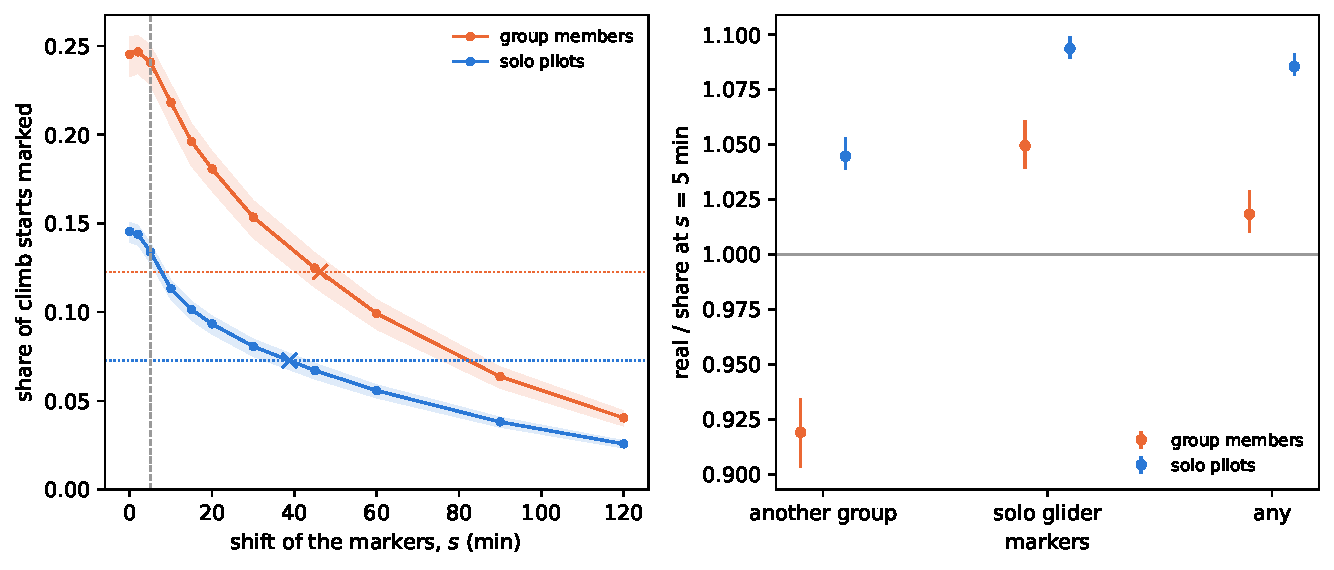
\includegraphics[width=\textwidth]{figures/structure/marking.pdf}
\caption{Thermal marking. Left: share $m(s)$ of the climb starts marked against the shift $s$ of the
markers, for group members and for solo pilots; dashed: $s_{\rm n}$; dotted and crosses: half of
$m(0)$ and $s_{1/2}$. Right: the ratio~\eqref{eq:now} by kind of marker. Bands and bars: 5--95\% of
200 draws of the dates.}
\label{fig:marking}
\end{figure}

\begin{itemize}
  \item \textbf{Group members meet a marker more often than solo pilots} (Figure~\ref{fig:marking},
        left): of \StMkGroupStarts{} climb starts of group members \StMkShareGroup\% are marked,
        and of \StMkSoloStarts{} of solo pilots \StMkShareSolo\%. The shifted markers give nearly as
        many.
  \item \textbf{A glider climbing right then adds little} (right): the ratio~\eqref{eq:now} is
        \StMkNowSolo{} \StMkNowSoloBand{} for solo pilots and \StMkNowGroup{} \StMkNowGroupBand{} for
        group members. For group members, markers of another group give \StMkNowGroupOther{}
        \StMkNowGroupOtherBand{} and solo gliders \StMkNowGroupSolo{} \StMkNowGroupSoloBand. The value
        below 1 stays open; one possibility is that groups flying one after the other along a route
        pass a thermal minutes apart, which the shifted markers keep.
  \item \textbf{Places keep producing climbs} (left): $m$ halves at $s_{1/2}=\StMkHalfGroup$~min for
        group members and \StMkHalfSolo~min for solo pilots. The shifted markers also leave their
        flights, so $s_{1/2}$ is an upper bound.
\end{itemize}
Limits. An excess over the null would be marking or two pilots finding one active thermal; the data
do not separate them. The test sees marking only from within about \StMkReach~km, the distance a
glider covers at \StMkGlideSpeed~km/h, the glide speed of solo pilots, in $T_{\rm m}$. A marker
seen from farther or longer ago is not tested: the ratio at large shifts grows mostly because the
shifted markers leave their flights, so we do not use it.

\subsubsection{Encounters}\label{sec:encounters}

When two gliders not in contact come close, how often do they join? A \emph{pass} is a maximal run
of grid instants at which two flights are within a horizontal distance $R_{\rm e}=\StEnR$~m, with no
pair interval of the run; $R_{\rm e}$ is the 95th percentile of the distance of the two flights at
the start of the pair intervals, beyond which few contacts begin. Runs of one pair separated by
less than the gap of the method are one. We keep the genuine approaches (the two were at least
$R_{\rm e}$ apart the instant before), the first meeting of the two units that day (no earlier contact between them),
and those with headings within $\theta_{\max}=\StEnTheta^\circ$ at the closest instant, since the
method links only gliders on similar headings. The unit of a glider is its group at the start of the
pass, or itself if solo, so a group meeting a glider is one pass and not one per member; $d_{\min}$
is the closest distance of a pair of members, and the height difference is that of the same pair
at that instant. The pass is \emph{joined} if a pair interval between a
member of one unit and a member of the other starts during the pass or within $\delta=\StEnDelta$~s
after its end: a contact that the method dates to the pass, since the glider behind reaches the
place of the other within $\delta$. There are \StEnPassesSoloSolo{}
passes of two solo gliders, \StEnPassesSoloGroup{} of a solo glider and a group and
\StEnPassesGroupGroup{} of two groups.

We follow $P(\text{joined})$ against $d_{\min}$ in \StEnBins{} bins of $\StEnBin$~m, with solo-solo as the
reference: groups attract if solo-group lies above it, and keep closed if group-group lies below.
Two ratios to the reference are read. The first, $\rho_x$, is the standardised ratio
\begin{equation}\label{eq:standard}
\rho_x=\frac{\sum_b w_b\,P_x(b)}{\sum_b w_b\,P_{ss}(b)},\qquad x=\text{solo-group, group-group},
\end{equation}
with $P_x(b)$ the share joined in the bin $b$ of $d_{\min}$ and $w_b$ the number of solo-solo
passes in it, so that the types are compared at the same distances. The second answers the number
of gliders: a unit of $n$ gliders meeting one of $m$ offers $nm$ pairs, and joins more often than two
solo gliders without any attraction. With $p(d_{\min})$ the solo-solo share joined in the bin, the
expected joins are
\begin{equation}\label{eq:chances}
E=\sum_{\text{passes}}\Big[1-\big(1-p(d_{\min})\big)^{nm}\Big],
\end{equation}
and we read the observed joins over $E$. Members fly together, so their chances are not
independent and $E$ is an upper bound on the part that the number of gliders gives alone: a ratio
above 1 is a lower bound on what is left.

\begin{figure}
\centering
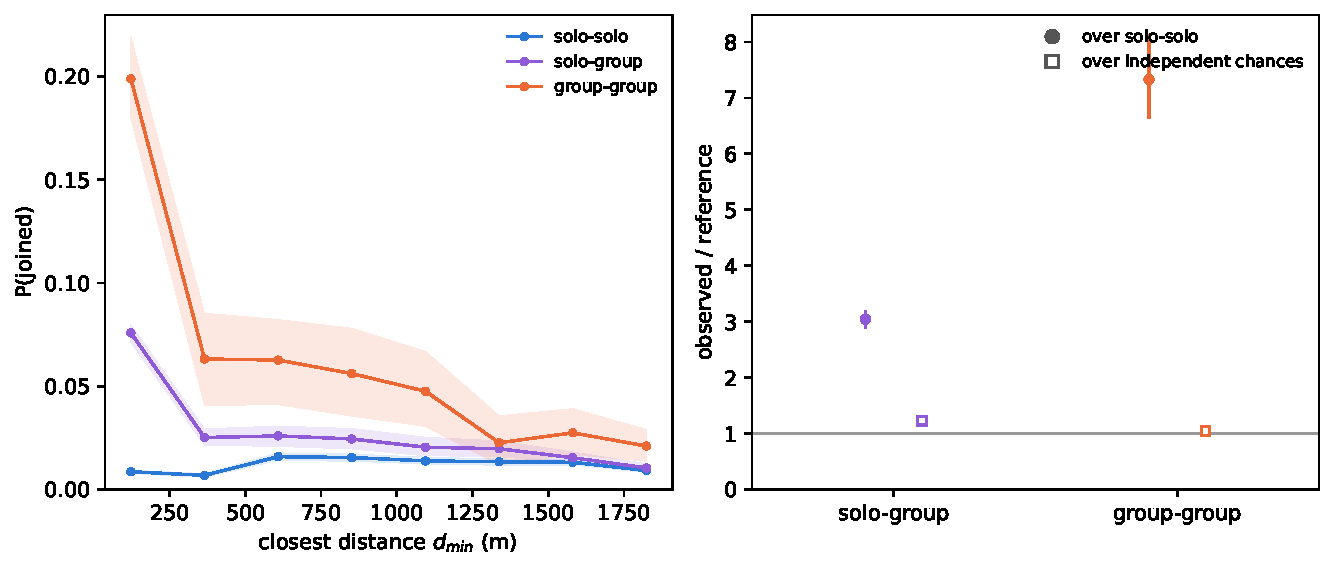
\includegraphics[width=\textwidth]{figures/structure/encounters.pdf}
\caption{Encounters of gliders not in contact. Left: share of the passes joined against the closest
distance $d_{\min}$, by type. Right: for solo-group and group-group, the standardised
ratio~\eqref{eq:standard} to solo-solo (full) and the observed joins over the independent
chances~\eqref{eq:chances} (open). Bands and bars: 5--95\% of 200 draws of the dates.}
\label{fig:encounters}
\end{figure}

\begin{itemize}
  \item \textbf{Groups are joined more often} (Figure~\ref{fig:encounters}, left): the share joined
        is \StEnShareSoloSolo\% for solo-solo, \StEnShareSoloGroup\% for solo-group and
        \StEnShareGroupGroup\% for group-group. It is flat in $d_{\min}$ for solo-solo and falls
        steeply for the others: for group-group \StEnNearGroupGroup\% below \StEnBin~m and
        \StEnFarGroupGroup\% at $R_{\rm e}$.
  \item \textbf{Most of it is the size of the target} (right): the standardised ratios are
        \StEnRatioSoloGroup{} \StEnRatioSoloGroupBand{} for solo-group and \StEnRatioGroupGroup{}
        \StEnRatioGroupGroupBand{} for group-group; over the independent chances they are
        \StEnObsExpSoloGroup{} \StEnObsExpSoloGroupBand{} and \StEnObsExpGroupGroup{}
        \StEnObsExpGroupGroupBand. Only a pair draws a solo glider a little more than its number gives
        (\StEnSoloPair{} \StEnSoloPairBand), a group of 3 or more does not (\StEnSoloThree{}
        \StEnSoloThreeBand).
  \item \textbf{Joining needs the same level}: of the solo-solo passes, \StEnBelowSoloSolo\% are
        joined when the height difference is at most $\varepsilon_z=\StEnEpsZ$~m and
        \StEnAboveSoloSolo\% above it. Above $\varepsilon_z$ the joins over the independent
        chances, taken in that class, are \StEnAboveSoloGroup{} \StEnAboveSoloGroupBand{} for
        solo-group and \StEnAboveGroupGroup{} \StEnAboveGroupGroupBand{} for group-group.
\end{itemize}

\paragraph{What we keep.} The gliders around a group add little for its pilots in these data.
A glider climbing right then adds little to the chance that a pilot starts to climb where it
climbs (ratios \StMkNowGroup{} and \StMkNowSolo), over a glider that climbed there minutes before
or after: places keep producing climbs, and that is what the shifted markers keep. Groups are
joined more often than solo gliders, and almost all of the excess is the number of gliders that a
group offers: a pair draws a solo glider a little more than its number gives, a group of 3 or more
draws one no more, and two groups join as often as their numbers give. Only uploaded tracks are
seen, so a marker or a glider that was not uploaded is missing.

\subsection{Pilots across days}\label{sec:days}

The names of the catalog link the flights of one pilot on different days. Do pilots choose their
partners (Section~\ref{sec:partners}), is that loyalty the habit of every pilot or of a core, how
much of it do the clubs hold, and who flies with whom (Section~\ref{sec:network})?

\subsubsection{With whom}\label{sec:partners}

Do pilots choose their partners, or fly with whoever is there? We follow paraglider pilots by their
name in the catalog (anonymised ones left out). Two pilots are partners on a day when their
flights share a pair interval: a \emph{pair-day}. Chance keeps who flies in a group where and
when: within each site-day (takeoffs within 3~km, joined when a pair interval links two sites),
the partners are redrawn at random, each pilot keeping its number of partners that day (a
configuration model; \StNwDraws{} draws). Where each of \StNwTries{} attempts to redraw a pool holds a pilot paired
with itself or the same pair twice, the pairs of the pool are mixed by swaps that keep every degree, so
each pilot keeps its number of pair-days in every draw. There are \StPairDays{} pair-days among \StPilots{} pilots and
\StPairs{} pairs; one pair flew together on \StMaxDays{} days (Figure~\ref{fig:partners}).
\begin{itemize}
  \item \textbf{Pilots return to the same partners:} \StRepeatObs\% of the pair-days are on pairs
        that meet on more than one day, against \StRepeatNull\% \StRepeatNullBand{} at random
        (\StRepeatPairsObs{} such pairs against \StRepeatPairsNull).
  \item \textbf{and to their club:} \StSameClubObs\% of the pair-days join two pilots of the same
        club, against \StSameClubNull\% \StSameClubNullBand.
\end{itemize}
Chance already fixes who flies in a group at each site and day, so the excess is the choice of
partner among the pilots there. Choosing where and when to fly with friends stays in chance here.

\begin{figure}
\centering
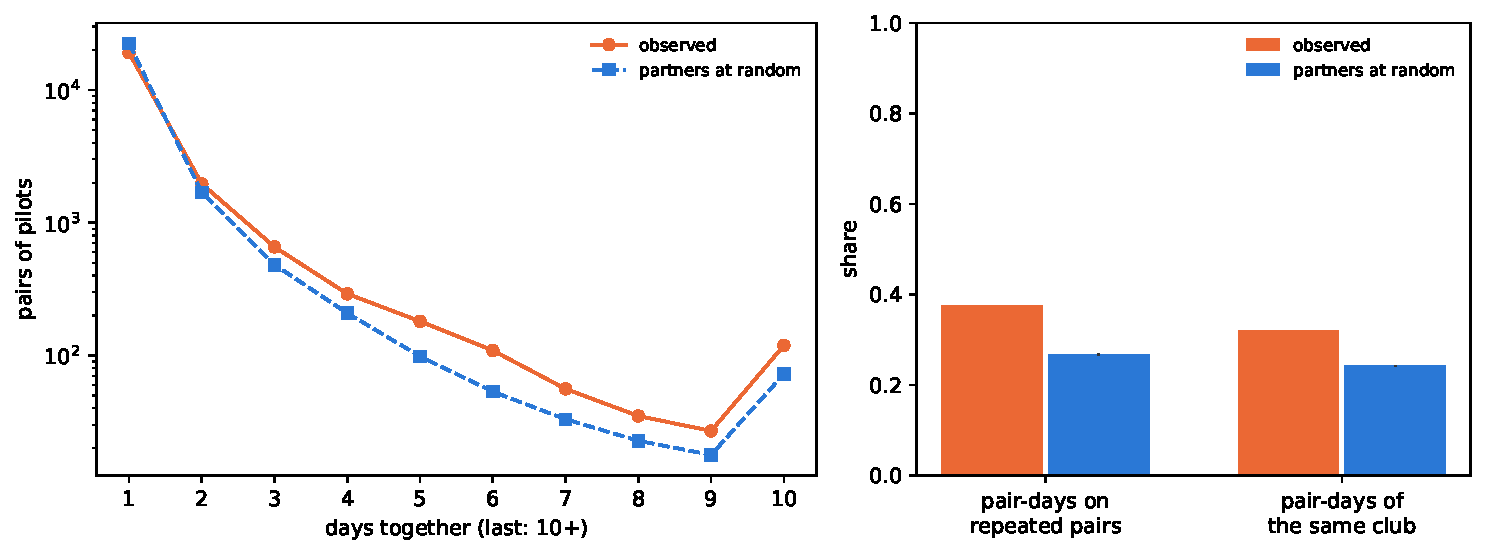
\includegraphics[width=0.85\textwidth]{figures/structure/partners.pdf}
\caption{Left: pairs of pilots by the number of days they flew together, observed and with
partners at random. Right: share of the pair-days on pairs that meet on more than one day, and of
two pilots of the same club (each pilot's main club); bars at random: 5--95\% of the draws.}
\label{fig:partners}
\end{figure}

\paragraph{Habitual leaders.} Pilots also differ in how they lead: some lead or follow in most of
their pairs, more than roles at random give: \HabitualExtreme\% lead in at most 20\% or at least 80\% of
their roles, against \HabitualExtremeNull\% expected (Section~\ref{sec:leaders},
Figure~\ref{fig:habitual} in Appendix~\ref{app:evidence}).

\subsubsection{Loyalty, clubs and likeness}\label{sec:network}

What does the loyalty above look like pilot by pilot, how much of it do the clubs hold, and who
flies with whom? The population and the null are those of Section~\ref{sec:partners}: the
pair-days of named paraglider pilots, and the partners redrawn within each pool of site-days
(\StNwDraws{} draws) with every pilot keeping its number $s$ of pair-days. Seen as a graph, the
pilots are the nodes and the pair-days the edges.

\paragraph{Loyalty of each pilot.} For the \StNwPilots{} pilots with $s\ge\StNwSMin$ pair-days, $k$
is the number of distinct partners over their $s$ pair-days, in the data and in each draw. The
randomized probability integral transform of the data among the $N$ draws is
\begin{equation}\label{eq:pit}
q=\frac{\#\{k_{\rm draw}<k\}+U\,\big(\#\{k_{\rm draw}=k\}+1\big)}{N+1},\qquad U\sim\mathrm{Uniform}(0,1).
\end{equation}
Without loyalty $k$ and the draws are exchangeable and $q$ is uniform, with density 1; loyalty,
fewer distinct partners than at random, moves $q$ toward 0. A general habit shifts the whole
histogram; a core of loyal pilots makes a spike at 0 over a flat rest. We split the pilots by their
$s$: $s\le\StNwEdgeLow$, $\StNwEdgeLow<s\le\StNwEdgeHigh$ and $s>\StNwEdgeHigh$.

\paragraph{Clubs.} A pair is repeated if it meets on two or more days. The excess of pair-days on
repeated pairs is the observed number minus the mean of the null, split by whether the two flights
of the day are of the same club or of different clubs (the club is unknown for a negligible share).

\paragraph{Likeness.} The experience $E$ of a pilot is its number of earlier flights in the catalog
at the date, taken as $x=\log_{10}(1+E)$ as in Section~\ref{sec:leaders}. Each pair-day counts in
both directions. We follow the mean $x$ of the partner against the own $x$ in deciles, and the
Pearson correlation of $x$ across the two ends. The same is done for the wing class (A~=~1 to
competition~=~5), with the share of pair-days in the same class. A curve above the null for
beginners would be mentoring; a steeper curve than the null is assortativity.

\begin{figure}
\centering
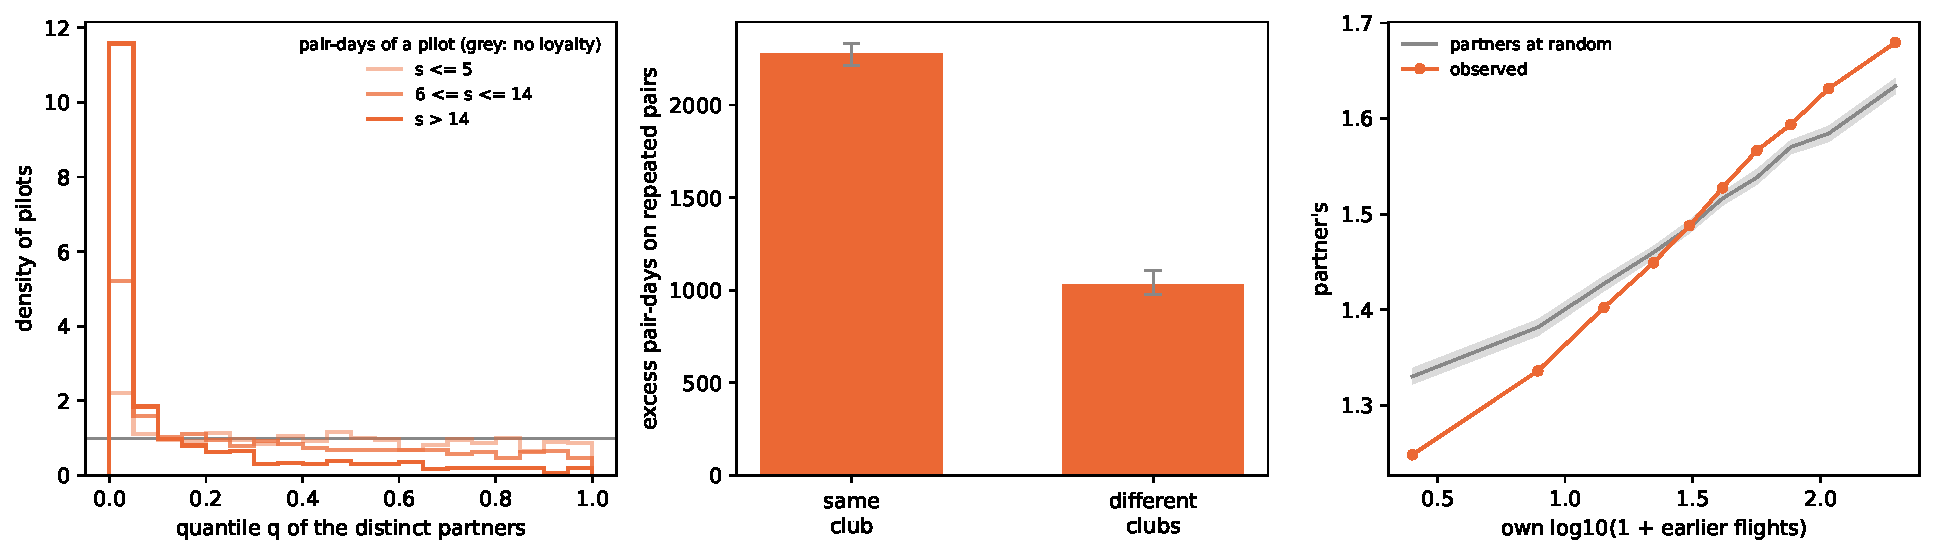
\includegraphics[width=\textwidth]{figures/structure/network.pdf}
\caption{Pilots across days. Left: histogram of the quantile $q$~\eqref{eq:pit} of the distinct
partners, by class of the number of pair-days of the pilot; grey line: no loyalty. Middle: excess of
pair-days on repeated pairs, observed minus partners at random, inside and outside clubs.
Right: mean $x$ of the partner against own $x$, observed and with partners at random. Bars and
band: 5--95\% of the \StNwDraws{} draws of the null; the observed values are points.}
\label{fig:network}
\end{figure}

\begin{itemize}
  \item \textbf{Loyalty grows with activity} (Figure~\ref{fig:network}, left): the share of pilots
        with $q<\StNwQLow$, \StNwQLow{} without loyalty, is \StNwLowFew\%, \StNwLowMid\% and
        \StNwLowMany\% in the three classes (\StNwPilotsFew, \StNwPilotsMid{} and \StNwPilotsMany{}
        pilots). Among the occasional pilots a spike at 0 over a flat rest, a small core; among the
        most active the whole histogram moves, with the median $k$ at \StNwRatioMany{} of its null
        value (\StNwRatioFew{} and \StNwRatioMid{} in the other classes, \StNwRatioNullMany{} in the
        draws).
  \item \textbf{Clubs hold most of the loyalty} (middle): the excess is
        \StNwExcessSame{} \StNwExcessSameBand{} pair-days inside the same club and
        \StNwExcessDiff{} \StNwExcessDiffBand{} between clubs, \StNwShareSame\% and \StNwShareDiff\%
        of it. Of the pair-days on repeated pairs \StNwRealSame\% are inside a club, against
        \StNwNullSame\% in the null: the clubs hold a little more than their share, and a third of the
        loyalty crosses clubs.
  \item \textbf{Pilots fly with pilots of their own experience} (right): the correlation of $x$
        across the two ends is \StNwCorrX, against \StNwCorrXNull{} \StNwCorrXNullBand{} at random.
        There is no mentoring: the partners of the least experienced decile have $x=\StNwBeginner$,
        against \StNwBeginnerNull{} \StNwBeginnerNullBand{} at random, and \StNwVeteran{} against
        \StNwVeteranNull{} \StNwVeteranNullBand{} in the most experienced.
  \item \textbf{The wing class is more alike still}: the correlation is \StNwCorrWing{} against
        \StNwCorrWingNull{} \StNwCorrWingNullBand, and \StNwSameWing\% of the pair-days are in one
        class, against \StNwSameWingNull\% \StNwSameWingNullBand. Similar wings may keep two gliders
        together longer through their speed: a hypothesis that these data do not test.
\end{itemize}

\paragraph{What we keep.} Pilots come back to the same partners, and the return is not the same for
everyone: a small core among the occasional pilots, the habit of most among the active ones. Clubs
hold most of it and a third crosses them. Pilots fly with pilots of a similar experience and
wing class more than who flies where and when gives, and beginners do not fly with the most
experienced more than chance gives. The names of the catalog are the limit: homonyms join, and a
pilot who changes name splits.

\subsection{What the data support}\label{sec:conclusions}

\paragraph{Two pilots} (Section~\ref{sec:pilots}).
\begin{itemize}
  \item group pilots keep the same pace: their delay wanders half as fast as that of two pilots
        kept in contact by chance, and they stay closer after the contact;
  \item in glide the follower turns where the head turned, the delay later (a peak at
        $\tau=\StHdPeakThree$~s for $\ell=\StHdLThree$~s), and no response at short lags appears;
        close pilots share the line more than chance pairs do;
  \item not supported: a spring that pulls pilots back, since the pull is about that of chance
        contacts selected the same way.
\end{itemize}

\paragraph{The group} (Section~\ref{sec:group}).
\begin{itemize}
  \item groups are mostly pairs; large ones are strings along the route that change members every
        few minutes, while the episode lasts about an hour;
  \item the size distribution follows from one pilot joining or leaving at a time; its heavy tail
        from members of larger groups leaving less often;
  \item the longer a pair has lasted, the less it separates, beyond lasting partnerships; joins
        come in the first minutes of an episode;
  \item in a thermal a group closes up like an accordion at fixed delays; in glide it opens after
        the thermal, along lines closer than those of chance pairs;
  \item the lead changes a few times per hour, mostly as the group enters or leaves a thermal,
        and goes more often to the experienced pilot on the higher wing; within a group no pilot
        holds it much longer than random hand-overs give;
  \item followers leave a thermal at about the leader's height, a few metres lower; who stays
        longer leaves higher, and the first to leave leads the next glide;
  \item not supported: that the shape of a group (triangle or chain, complete or tree) changes how
        its pilots fly; a social rank from the order in a group, since a line along the route is
        geometry; a life cycle of the episode, since members do not leave more as it ages; that
        height gained in a thermal gives the lead; a fan that opens across the route to search in
        glide and closes before the next thermal.
\end{itemize}

\paragraph{Between groups} (Section~\ref{sec:between}).
\begin{itemize}
  \item a glider climbing right then adds little to the chance that a pilot starts to climb where
        it climbs: the ratio to markers shifted by \StMkNear~min is \StMkNowGroup{} for group
        members and \StMkNowSolo{} for solo pilots;
  \item groups are joined more often than solo gliders, and almost all of the excess is the number
        of gliders a group offers: over independent chances \StEnObsExpSoloGroup{} for solo-group and
        \StEnObsExpGroupGroup{} for group-group passes.
\end{itemize}

\paragraph{Pilots across days} (Section~\ref{sec:days}).
\begin{itemize}
  \item pilots return to the same partners and to their club mates more than who flies where and
        when explains; loyalty is a small core among the occasional pilots and the habit of most
        of the active ones, and \StNwShareDiff\% of its excess pair-days cross clubs;
  \item pilots fly with pilots of a similar experience and wing class more than chance gives, and
        beginners are not paired with veterans more than chance gives.
\end{itemize}

\paragraph{What the data cannot tell.}
\begin{itemize}
  \item whether the shared pace is following: the surrogate pairs fly at another hour, and a
        follower who retraces the head's track gives the same signal as two pilots in the same air;
  \item whether a start that follows a marker is marking or two pilots finding one active thermal;
        the test sees marking only from within about \StMkReach~km, and only uploaded tracks are
        seen, so the neighbours are undercounted and the effects diluted;
  \item whether the likeness in wing class is physical, similar speeds keeping two gliders
        together longer;
  \item who a pilot is beyond the name of the catalog: homonyms join, a pilot who changes name
        splits.
\end{itemize}

\medskip
One caveat: in a thermal the altitude fixes $\ell^*(t)$ to about a turn, 20~s
(Appendix~\ref{gi-sec:lag} of the note), for real and chance contacts alike, so the cohesion and the switches of
the lead carry this noise on both sides of the comparison with chance.
